\chapter{Étude technique}
\label{chap-etude-technique}

Ce chapitre décrit la solution ARGOS telle qu'elle est réellement implémentée.
L'analyse a porté sur le micrologiciel ESP32, les routes Flask, les services
métier, les scripts de l'interface, les migrations SQL, le schéma PostgreSQL
actif et l'orchestration Docker. Cette démarche permet de faire correspondre
les diagrammes aux composants exécutables et d'éviter de présenter comme
opérationnelle une fonction qui ne serait qu'envisagée.

Le chapitre répond à quatre questions : quels acteurs utilisent ARGOS, comment
l'application est-elle organisée, comment une mesure devient-elle une donnée
visible et durable, et quelles structures garantissent son identité, sa
sécurité et sa traçabilité ?

\section{Analyse}

Cette section ouvre l'étude technique du projet ARGOS en formalisant l'ensemble des besoins auxquels la solution doit répondre. Elle distingue les besoins fonctionnels, qui décrivent les services attendus du système, des besoins non fonctionnels, qui définissent les contraintes de performance, de sécurité et de robustesse à respecter. Cette étape est indispensable car elle constitue le socle sur lequel reposent tous les choix de conception présentés dans la suite du chapitre.

\subsection{Analyse des besoins}

L'analyse des besoins a pour objectif de formaliser, de manière exhaustive et structurée, l'ensemble des exigences auxquelles la solution ARGOS doit répondre pour garantir la continuité numérique du fret, assurer l'interopérabilité des données et offrir une base juridique fiable en cas de litige. Elle repose sur une distinction fondamentale entre les besoins fonctionnels (les services rendus par le système) et les besoins non fonctionnels (les contraintes de performance, de sécurité et de robustesse). Cette analyse intègre les exigences réglementaires de l'OMI applicables depuis janvier~2026 et s'adapte aux contraintes opérationnelles des corridors logistiques d'Afrique centrale. Sa traduction technique formalisée fait l'objet de la \cref{sec-specifications} de ce chapitre.

\subsubsection{Besoins fonctionnels}

Classés selon la méthode MoSCoW, ces besoins définissent les fonctionnalités du système en priorisant la livraison d'un Produit Minimum Viable (MVP) orienté vers la transparence et la déconnexion des silos d'information.

\begin{itemize}
\item \textbf{Télémesure et acquisition Edge horodatée}~: collecte en continu (intervalle de 5~minutes) et traitement à la périphérie (Edge Computing) des données d'intégrité physique~: température (précision $\pm$0,2~°C), humidité (précision $\pm$2~\%), chocs et vibrations tridimensionnels, luminosité pour la détection instantanée d'ouverture de porte. Chaque mesure est obligatoirement associée à un horodatage UTC précis.
\item \textbf{Géolocalisation continue par inertie}~: suivi spatial en temps réel via le module NEO-M8U. En cas de perte du signal satellite (cale de navire, entrepôt, tunnel), le système bascule sur l'estimation de position par inertie (UDR~--~Untethered Dead Reckoning) pour maintenir la continuité de la trajectoire\cite{ublox}.
\item \textbf{Passerelle de communication hybride}~: transmission des données de manière dynamique via les réseaux cellulaires IoT (LTE-M, NB-IoT) en routage normal, par Wi-Fi pour la collecte automatique de proximité en zone portuaire (PAD/PAK), et par connexion physique (USB/RJ45) comme canal de secours pour les audits techniques.
\item \textbf{Plateforme SaaS de supervision multi-locataire}~: déploiement d'un tableau de bord web structuré selon six profils de responsabilité (client/chargeur, entreprise utilisatrice, propriétaire, transporteur, autorité portuaire et superadministrateur), avec gestion des accès par jetons Bearer signés et horodatés, cartographie dynamique (Leaflet.js) et notifications applicatives et e-mail lors d'une rupture de scellé ou d'une excursion thermique.
\end{itemize}

\begin{itemize}
\item \textbf{Génération de rapports d'anomalies certifiés}~: exportation automatisée de documents PDF horodatés et cryptographiquement intègres, conçus pour servir de rapports d'expertise directement opposables auprès des compagnies d'assurance et des tribunaux de commerce en cas de litige.
\item \textbf{Monétisation et gestion des abonnements}~: module d'administration permettant aux agences propriétaires de gérer la flotte de boîtes noires et d'affecter des droits d'accès temporaires ou récurrents aux agences utilisatrices selon une logique d'abonnement.
\end{itemize}

\begin{itemize}
\item \textbf{Passerelle de paiement intégrée}~: la facturation et le traitement des abonnements se feront hors ligne pour la version de lancement.
\item \textbf{Localisation internationale multilingue complète}~: l'interface de la plateforme sera exclusivement restreinte au français et à l'anglais pour la première version industrielle.
\end{itemize}

\subsubsection{Besoins non fonctionnels}

Ils fixent les critères de qualité, de sécurité informatique et de robustesse industrielle indispensables pour valider la confiance des opérateurs maritimes dans la solution ARGOS.

\begin{itemize}
\item \textbf{Fluidité de l'API}~: temps de réponse global inférieur à 500~millisecondes au 95\textsuperscript{e}~percentile.
\item \textbf{Priorisation des files d'attente (QoS)}~: transmission standard toutes les 15~minutes en régime normal, basculement en mode d'alerte instantané (latence inférieure à 10~secondes) dès la détection d'un événement critique.
\item \textbf{Rendu cartographique}~: chargement et affichage de plus de 100~marqueurs de conteneurs actifs en moins de 2~secondes.
\item \textbf{Montée en charge}~: architecture backend supportant 1~000~boîtes noires communicantes simultanément, sans dégradation des performances.
\end{itemize}

\begin{itemize}
\item \textbf{Chiffrement de bout en bout}~: sécurisation de l'ensemble des flux par le protocole TLS~1.3.
\item \textbf{Contrôle d'accès strict (RBAC)}~: authentification par jetons Bearer signés et horodatés, associée à un contrôle d'accès basé sur les rôles et le périmètre effectif des ressources.
\item \textbf{Intégrité du matériel (firmware)}~: signature cryptographique obligatoire du micrologiciel et déploiement des mises à jour à distance (OTA) via un canal sécurisé.
\end{itemize}

\begin{itemize}
\item \textbf{Étanchéité extrême}~: certification IP67 obligatoire (étanchéité totale aux poussières, résistance à l'immersion temporaire à 1~mètre selon la norme IEC~60529).
\item \textbf{Résilience mécanique et thermique}~: absorption de chocs accidentels jusqu'à 50g, plage de fonctionnement thermique industriel de $-20$~°C à $+70$~°C.
\item \textbf{Légalité et persistance à long terme}~: rétention et immuabilité des données historiques sur le Cloud pendant un minimum de 3~ans, en conformité avec les obligations d'audit de l'OMI.
\end{itemize}

\begin{itemize}
\item \textbf{Furtivité morphologique}~: facteur de forme ultra-compact limité à 15~cm $\times$ 10~cm $\times$ 5~cm maximum, teintes neutres, préservant 100~\% du volume utile de chargement.
\item \textbf{Accessibilité multiplateforme}~: interface web responsive optimisée de 360~pixels (smartphones des chauffeurs) à 1920~pixels (écrans des terminaux portuaires).
\end{itemize}

\subsection{Spécifications des besoins}
\label{sec-specifications}
Nous allons tout d'abord traduire les besoins exprimés en spécifications techniques strictes et codifiées, lesquelles serviront de référence tout au long de la conception et de la recette du système. Cette démarche décrit, d'une part, les fonctionnalités métiers que le système ARGOS doit exécuter (besoins fonctionnels, codifiés SF) et, d'autre part, les exigences de qualité, de sécurité et d'environnement auxquelles le dispositif doit se conformer (besoins non fonctionnels, codifiés NF).

\subsubsection{Spécifications des besoins fonctionnels (SBF)}

L'ensemble des fonctionnalités métiers indispensables au fonctionnement et à la supervision de la solution ARGOS est synthétisé dans le Tableau~\ref{tab:spec_fonctionnelles}.

\begin{xltabular}{\textwidth}{@{}p{1.4cm} p{3.0cm} X p{1.8cm}@{}}
\caption{Spécifications des besoins fonctionnels (SBF)} \label{tab:spec_fonctionnelles} \\
\toprule
\tableheadrow \thc{Code} & \thc{Fonctionnalité} & \thc{Description technique et métrique cible} & \thc{Priorité} \\
\midrule
\endfirsthead
\toprule
\tableheadrow \thc{Code} & \thc{Fonctionnalité} & \thc{Description technique et métrique cible} & \thc{Priorité} \\
\midrule
\endhead
\endfoot
\bottomrule
\multicolumn{4}{l}{\textit{Source : Les Promoteurs 2025-2026}} \\
\endlastfoot
\textbf{SF-01} & Télémesure multisensorielle & Acquisition automatique toutes les 5~min des données internes~: température ($\pm$0,2~°C), humidité ($\pm$2~\%), luminosité (détection d'ouverture), chocs tridimensionnels (jusqu'à 16g). Chaque mesure inclut un horodatage UTC. & Must have \\
\hline
\textbf{SF-02} & Géolocalisation par inertie & Calcul de la position via le module GPS/GNSS NEO-M8U. En l'absence de signal, basculement automatique sur l'estimation par inertie (Dead Reckoning). & Must have \\
\hline
\textbf{SF-03} & Stockage Edge résilient & Sauvegarde locale en zone blanche~: mémoire FRAM pour l'écriture instantanée des alertes critiques, Flash SPI pour l'historique complet. Synchronisation prioritaire au retour du réseau. & Must have \\
\hline
\textbf{SF-04} & Communication hybride & Routage adaptatif~: cellulaire IoT (LTE-M/NB-IoT) en transit, Wi-Fi pour le déchargement massif en zone portuaire, liaison physique USB/RJ45 pour la maintenance. & Must have \\
\hline
\textbf{SF-05} & API REST d'interopérabilité & Point d'accès unique sécurisé pour le partage des flux de données brutes d'ARGOS vers les systèmes tiers (TOS portuaires, systèmes douaniers, ERP). & Must have \\
\hline
\textbf{SF-06} & Plateforme SaaS de supervision & Interface web multi-profils (Client, Agence, Chauffeur, SuperAdmin) avec cartographie dynamique (Leaflet.js) et notifications applicatives. & Must have \\
\hline
\textbf{SF-07} & Gestion basse consommation & Algorithme d'économie d'énergie (mode Deep Sleep), consommation sous 1~mA hors émission, 90~jours d'autonomie sur batterie 10~000~mAh. & Must have \\
\hline
\textbf{SF-08} & Rapports d'avarie certifiés & Génération automatique de rapports PDF cryptographiquement intègres, opposables auprès des assurances et tribunaux. & Should have \\
\hline
\textbf{SF-09} & Mode avion local & Suspension temporaire des émissions radiofréquences depuis la cabine du chauffeur, sans interrompre l'enregistrement local. & Should have \\
\end{xltabular}

\noindent \textbf{Bilan et portée analytique~:} 
Le Tableau~\ref{tab:spec_fonctionnelles} structure l'architecture fonctionnelle de la solution ARGOS en définissant précisément les services offerts par le système. De l'acquisition multisensorielle en temps réel à la restitution sur la plateforme SaaS en passant par la résilience en zone blanche, ce référentiel garantit que l'ensemble des besoins métiers des armateurs et des chargeurs est couvert de manière rigoureuse, constituant ainsi le cahier des charges technique de référence pour le développement et la phase de test.

\subsubsection{Spécifications des besoins non fonctionnels (SBNF)}

Les exigences de qualité, de robustesse matérielle et de sécurité informatique indispensables à la crédibilité industrielle du projet sont regroupées dans le Tableau~\ref{tab:spec_non_fonctionnelles}.

\begin{xltabular}{\textwidth}{@{}p{1.4cm} p{3.0cm} X@{}}
\caption{Spécifications des besoins non fonctionnels (SBNF)} \label{tab:spec_non_fonctionnelles} \\
\toprule
\tableheadrow \thc{Code} & \thc{Catégorie} & \thc{Exigence technique et indicateur de performance (KPI)} \\
\midrule
\endfirsthead
\toprule
\tableheadrow \thc{Code} & \thc{Catégorie} & \thc{Exigence technique et indicateur de performance (KPI)} \\
\midrule
\endhead
\endfoot
\bottomrule
\multicolumn{3}{l}{\textit{Source : Les Promoteurs 2025-2026}} \\
\endlastfoot
\textbf{NF-01} & Performance API & Temps de réponse de l'API REST inférieur à 500~ms au 95\textsuperscript{e}~percentile. \\
\textbf{NF-02} & Réactivité (QoS) & Latence inférieure à 5~secondes entre la détection d'une alerte critique (choc $>$8g, ouverture) et sa réception sur la plateforme. \\
\textbf{NF-03} & Scalabilité & Le backend doit absorber les connexions simultanées de 1~000~boîtiers sans perte de paquets. \\
\textbf{NF-04} & Sécurité des flux & Chiffrement obligatoire de toutes les communications via TLS~1.3. \\
\textbf{NF-05} & Contrôle d'accès & Authentification JWT (expiration 15~min) et architecture RBAC isolant les données entre concurrents. \\
\textbf{NF-06} & Sécurité du matériel & Signature cryptographique du firmware et sécurisation des mises à jour OTA. \\
\textbf{NF-07} & Étanchéité & Certification IP67 (poussière totale, immersion temporaire 1~m / 30~min, norme IEC~60529). \\
\textbf{NF-08} & Résistance mécanique & Chocs et impacts accidentels jusqu'à 50g sans altération des composants internes. \\
\textbf{NF-09} & Tolérance thermique & Plage de fonctionnement nominale de $-20$~°C à $+70$~°C. \\
\textbf{NF-10} & Légalité et persistance & Persistance et immuabilité des données de transit sur 3~ans minimum, conformité OMI. \\
\textbf{NF-11} & Furtivité morphologique & Dimensions maximales 15~$\times$~10~$\times$~5~cm, coloris neutre, espace de chargement préservé. \\
\textbf{NF-12} & Compatibilité applicative & Responsive Design de 360~px à 1920~px, compatible deux dernières versions de Chrome, Firefox, Safari et Edge. \\
\end{xltabular}

\noindent \textbf{Bilan et portée analytique~:} 
Le Tableau~\ref{tab:spec_non_fonctionnelles} vient encadrer les conditions d'exploitation du système en fixant des indicateurs de performance (KPI) stricts. En combinant des exigences de haute disponibilité logicielle (temps de réponse API, scalabilité cloud, chiffrement TLS 1.3) et de robustesse matérielle en conditions extrêmes (norme IP67, résistance aux chocs de 50g, plage thermique de $-20$~°C à $+70$~°C), ces spécifications garantissent la fiabilité opérationnelle du dispositif sur les corridors terrestres et maritimes d'Afrique centrale.

\section{Conception générale}

Cette partie présente les grandes orientations retenues pour la réalisation du système ARGOS. Elle expose la méthodologie de développement adoptée, l'environnement technologique choisi ainsi que les principaux choix logiciels et matériels effectués, en justifiant chacune de ces décisions. Elle donne ainsi une vue d'ensemble de la manière dont le projet a été pensé et structuré, avant que les aspects plus techniques ne soient détaillés dans la section suivante.

\subsection{Méthodologie de développement : l'approche hybride V-DSDM}
\label{sec-methodologie-v-dsdm}

Pour mener à bien la conception et la réalisation du système ARGOS, qui allie une composante matérielle (le dispositif embarqué) et une plateforme logicielle dynamique (API, interface web, base de données), nous avons opté pour une méthodologie hybride : le modèle \textbf{V-DSDM} (Cycle en V couplé à la méthode Agile DSDM).

\subsubsection{Justification du choix méthodologique (Le « Pourquoi »)}

Afin d'optimiser le processus de réalisation du projet, une démarche méthodologique hybride a été adoptée, dissociant le cycle de développement matériel et logiciel selon les modalités suivantes :
\begin{itemize}
    \item \textbf{Pour le dispositif matériel (Cycle en V) :} La conception électronique et matérielle (ESP32, capteurs MPU6050, DHT22, circuits d'alimentation) nécessite une approche prédictive et séquentielle. Une erreur de conception matérielle ou un mauvais choix de composant entraîne des coûts de refabrication élevés et des délais incompressibles. Le modèle en V est donc idéal, car il impose une descente rigoureuse (analyse, spécification, architecture) avant toute réalisation, garantissant que les tests de validation ascendants répondront exactement aux exigences initiales.
    \item \textbf{Pour la plateforme logicielle (DSDM) :} Le développement de l'interface web, du backend Flask et des algorithmes de traitement de données requiert de l'adaptabilité. La méthode Agile DSDM (\emph{Dynamic Systems Development Method}) permet de livrer des fonctionnalités par itérations successives (MoSCoW : \emph{Must have, Should have, Could have, Won't have}), d'intégrer rapidement les retours utilisateurs et de s'adapter aux évolutions des protocoles de communication.
\end{itemize}
La fusion de ces deux approches en un modèle \textbf{V-DSDM} permet d'orchestrer la stabilité matérielle avec l'agilité logicielle.

\subsubsection{Déroulement de la procédure (Le « Comment »)}

Le développement s'articule autour d'une synchronisation entre les phases séquentielles du matériel et les itérations du logiciel, illustrées par la \cref{fig-methode-v-dsdm}.

\begin{enumerate}
    \item \textbf{Phase de descente (Analyse et Conception) :}
    Cette première étape séquentielle pose les fondations théoriques et structurelles du projet à travers les actions suivantes :
    \begin{itemize}
        \item \emph{Spécifications fonctionnelles et techniques :} Définition des besoins globaux du système (périmètre matériel et logiciel).
        \item \emph{Conception architecturale :} Séparation stricte des interfaces de communication (API, requêtes HTTP/MQTT) qui serviront de contrat entre le matériel et le logiciel.
        \item \emph{Conception détaillée (Matériel) :} Choix des capteurs, schémas électroniques, routage PCB.
    \end{itemize}
    
    \item \textbf{Phase de réalisation et Itérations DSDM :}
    Cette phase opérationnelle concrétise le développement en synchronisant les travaux physiques et logiciels selon l'organisation ci-dessous :
    \begin{itemize}
        \item \emph{Côté Matériel (Le fond du V) :} Assemblage du prototype physique, soudure, et écriture du firmware de bas niveau (gestion des capteurs).
        \item \emph{Côté Logiciel (Boucles itératives) :} Développement par « Timeboxes » (sprints). L'équipe logicielle utilise des maquettes de données (mocks) simulant le boîtier pour avancer sur l'API et le tableau de bord sans attendre la fin de la fabrication physique.
    \end{itemize}
    
    \item \textbf{Phase de remontée (Intégration et Validation) :}
    Cette ultime étape ascendante permet de vérifier la conformité globale du système déployé au travers des paliers de contrôle suivants :
    \begin{itemize}
        \item \emph{Tests d'intégration matériels-logiciels :} Le dispositif physique remplace les simulateurs. On valide la remontée réelle de la télémétrie vers le cloud.
        \item \emph{Validation système :} Test en conditions réelles (boîtier dans un conteneur en mouvement) vérifiant l'autonomie, la connectivité et la pertinence du tableau de bord.
    \end{itemize}
\end{enumerate}


% -----------------------------------------------------------------
% DIAGRAMME TIKZ DU MODÈLE V-DSDM (V étiré, police optimisée)
% -----------------------------------------------------------------
\begin{figure}[htbp]
\centering
\resizebox{0.92\textwidth}{!}{%
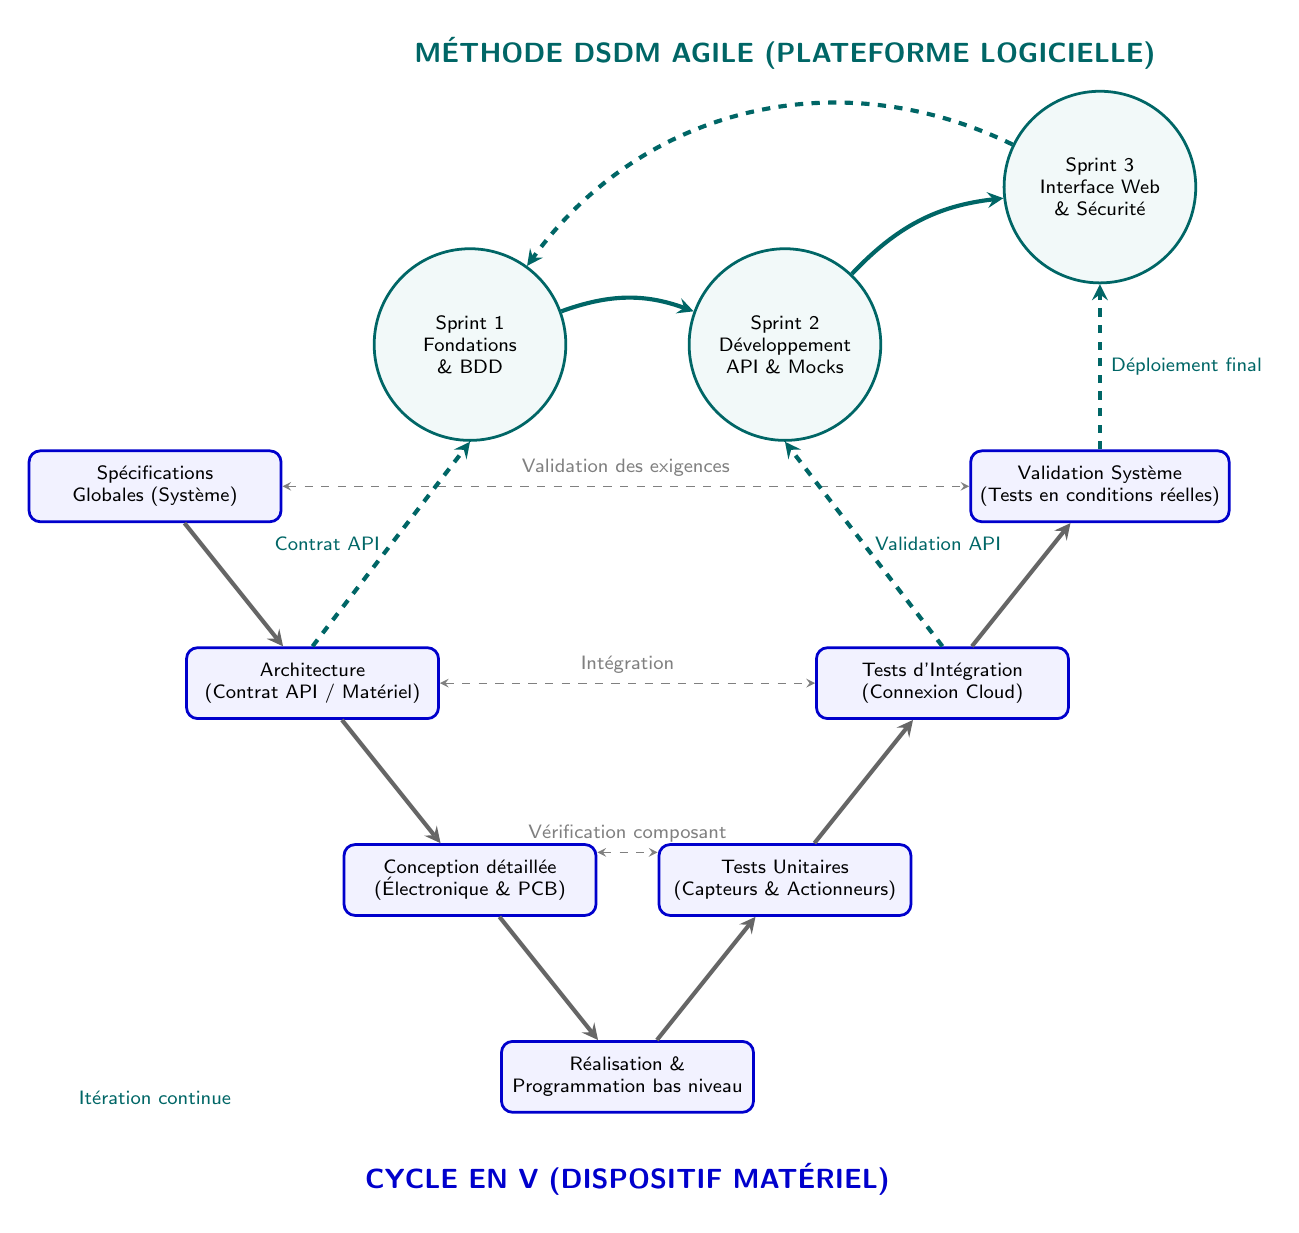
\begin{tikzpicture}[
  >=stealth,
  font=\sffamily\scriptsize,
  vnode/.style={draw=blue!80!black, rounded corners=4pt, fill=blue!5, 
                minimum width=3.2cm, minimum height=0.9cm, align=center, line width=1pt},
  agilenode/.style={draw=teal!80!black, circle, fill=teal!5, 
                    minimum width=2.2cm, align=center, line width=1pt, text width=2.0cm},
  arrow/.style={draw=gray!80!black, line width=1.5pt, ->},
  dashedarrow/.style={draw=gray!80!black, dashed, line width=1.2pt, <->}
]

% Branche descendante (V-Model Matériel) - Étirée en largeur et en profondeur
\node[vnode] (spec) at (0, 8) {Spécifications\\Globales (Système)};
\node[vnode] (archi) at (2, 5.5) {Architecture\\(Contrat API / Matériel)};
\node[vnode] (design) at (4, 3) {Conception détaillée\\(Électronique \& PCB)};
\node[vnode] (build) at (6, 0.5) {Réalisation \&\\Programmation bas niveau};

% Branche ascendante (V-Model Matériel)
\node[vnode] (testu) at (8, 3) {Tests Unitaires\\(Capteurs \& Actionneurs)};
\node[vnode] (testi) at (10, 5.5) {Tests d'Intégration\\(Connexion Cloud)};
\node[vnode] (valid) at (12, 8) {Validation Système\\(Tests en conditions réelles)};

% Itérations DSDM (Logiciel)
\node[agilenode] (sprint1) at (4, 9.8) {Sprint 1\\Fondations\\\& BDD};
\node[agilenode] (sprint2) at (8, 9.8) {Sprint 2\\Développement\\API \& Mocks};
\node[agilenode] (sprint3) at (12, 11.8) {Sprint 3\\Interface Web\\\& Sécurité};

% Flèches Cycle en V
\draw[arrow] (spec) -- (archi);
\draw[arrow] (archi) -- (design);
\draw[arrow] (design) -- (build);
\draw[arrow] (build) -- (testu);
\draw[arrow] (testu) -- (testi);
\draw[arrow] (testi) -- (valid);

% Validation croisée V
\draw[dashedarrow, thin, gray] (spec.east) -- (valid.west) node[midway, above] {\scriptsize Validation des exigences};
\draw[dashedarrow, thin, gray] (archi.east) -- (testi.west) node[midway, above] {\scriptsize Intégration};
\draw[dashedarrow, thin, gray] ([yshift=10pt]design.east) -- ([yshift=10pt]testu.west) node[midway, above] {\scriptsize Vérification composant};

% Flèches DSDM
\draw[arrow, teal!80!black] (sprint1) to[bend left=20] (sprint2);
\draw[arrow, teal!80!black] (sprint2) to[bend left=20] (sprint3);
\draw[arrow, teal!80!black, dashed] (sprint3) to[bend right=40] (sprint1) node[midway, above] {\scriptsize Itération continue};

% Liaisons V <-> DSDM
\draw[arrow, dashed, teal!80!black] (archi.north) -- (sprint1.south) node[midway, left, align=right] {\scriptsize Contrat API};
\draw[arrow, dashed, teal!80!black] (testi.north) -- (sprint2.south) node[midway, right] {\scriptsize Validation API};
\draw[arrow, dashed, teal!80!black] (valid.north) -- (sprint3.south) node[midway, right] {\scriptsize Déploiement final};

% Titres des zones
\node[font=\sffamily\normalsize\bfseries, text=blue!80!black] at (6, -0.8) {CYCLE EN V (DISPOSITIF MATÉRIEL)};
\node[font=\sffamily\normalsize\bfseries, text=teal!80!black] at (8, 13.5) {MÉTHODE DSDM AGILE (PLATEFORME LOGICIELLE)};

\end{tikzpicture}%
}
\caption{Schéma conceptuel de la méthodologie hybride V-DSDM appliquée au projet ARGOS}
\label{fig-methode-v-dsdm}
\tablesourcepromoteurs
\end{figure}
% -----------------------------------------------------------------

\subsubsection{Avantages de l'approche hybride}

L'adoption de cette méthodologie hybride, combinant la rigueur du cycle en V et l'adaptabilité de l'approche Agile DSDM, procure des bénéfices décisifs pour la réussite du projet ARGOS, lesquels se déclinent à travers les aspects suivants :

\begin{itemize}
    \item \textbf{Maîtrise des risques matériels :} La descente du modèle en V garantit que l'assemblage électronique de la boîte noire (cartes, alimentation, soudures) est pensé dans sa globalité avant la production, évitant les surcoûts matériels.
    \item \textbf{Réduction du \emph{Time-to-Market} :} Grâce à l'agilité logicielle (DSDM), le développement du tableau de bord web démarre en parallèle de la conception électronique. 
    \item \textbf{Qualité de l'intégration :} La définition précoce du contrat d'interface (Endpoints API, format JSON des trames MQTT) lors de la conception architecturale permet aux développeurs web de travailler avec de fausses données (mocks) en attendant la fin de la programmation de l'ESP32.
\end{itemize}

\subsubsection{Limites et défis d'implémentation}

Bien que performant et structurant pour le projet, ce modèle hybride n'est pas exempt de difficultés. La confrontation entre la rigueur séquentielle du matériel et l'agilité du logiciel soulève des défis opérationnels majeurs qu'il convient d'anticiper à travers les aspects suivants :

\begin{itemize}
    \item \textbf{Désynchronisation des rythmes :} L'agilité logicielle est rapide, tandis que la production matérielle (attente de livraison de composants, impression des PCB) subit des latences physiques. Si le matériel prend du retard, les tests d'intégration du logiciel sont bloqués.
    \item \textbf{Rigidité matérielle face aux pivots :} Si les itérations logicielles font émerger un nouveau besoin fonctionnel non prévu à l'origine (exemple : ajout d'un capteur biométrique de dernière minute), le modèle en V matériel est très rigide pour l'incorporer sans devoir recommencer la phase de conception électronique.
    \item \textbf{Complexité de la communication :} L'équipe doit jongler avec deux cultures de gestion de projet (documentation stricte pour l'électronique \emph{vs} pragmatisme et rapidité pour le web), ce qui demande une excellente coordination.
\end{itemize}


\subsection{Environnement technologique}

L'aboutissement technique et opérationnel du projet ARGOS repose sur la sélection rigoureuse d'un écosystème matériel et logiciel à la fois performant, sécurisé et interopérable. Afin de répondre aux exigences spécifiques de la télémétrie intelligente et du suivi logistique en temps réel, l'architecture technologique s'articule autour de choix structurels assumés. Les sections suivantes détaillent la nature de ces composantes ainsi que les justifications techniques et économiques qui ont motivé leur adoption.

\subsection{Choix logiciels et matériels}

La mise en œuvre concrète du système ARGOS mobilise une brique technologique diversifiée, allant du boîtier embarqué aux services Cloud. L'ensemble des solutions matérielles et logicielles retenues pour le développement et le déploiement du prototype est synthétisé dans le Tableau~\ref{tab-technologies-argos}.

\begin{table}[htbp]
\centering
\caption{Technologies effectivement mobilisées dans ARGOS}
\label{tab-technologies-argos}
\begin{tabularx}{\textwidth}{@{}p{3.2cm}p{3.7cm}X@{}}
\tableheadrow \thc{Composant} & \thc{Technologie} & \thc{Rôle effectif} \\
\midrule
Backend & Python 3.12, Flask, Gunicorn & Pages web, API utilisateur, API IoT et exécution WSGI \\
\hline
Accès aux données & Flask-SQLAlchemy, SQLAlchemy textuel & Connexions, transactions et requêtes SQL paramétrées \\
\hline
Base durable & PostgreSQL sur image TimescaleDB 14 & Données métier, télémétrie, audit, documents et tâches différées \\
\hline
Temps réel & Redis 7 & DB0 pour la limitation de débit ; DB1 pour la dernière mesure et le stream IoT \\
\hline
Interface & Jinja, HTML5, CSS3, JavaScript & Navigation par rôle, formulaires, pont direct et consommation des API \\
\hline
Visualisation & Leaflet, Chart.js & Carte, marqueurs, trajets, indicateurs et séries temporelles \\
\hline
Prototype & ESP32-S3, Arduino/C++ & Acquisition, point d'accès, stockage local, télémétrie et commandes \\
\hline
Protocoles & HTTP REST, JSON, CORS ; MQTT configurable & HTTP est utilisé par le prototype ; MQTT demeure un transport de commandes configurable \\
\hline
Déploiement & Docker Compose & Services \code{web}, \code{db}, \code{redis}, \code{worker} et \code{cloudflared} \\
\hline
Publication distante & Cloudflare Tunnel en HTTP/2 & URL HTTPS de démonstration sans exposition directe du routeur \\
\hline
Notifications & SMTP ou Infobip & Courriel et, selon la configuration, WhatsApp \\
\hline
Intégrations & BIC/BoxTech, suivi maritime, Gemini & Classification, enrichissement de voyage et assistant applicatif \\
\tablebottomrule
\end{tabularx}
\tablesourcepromoteurs
\end{table}

\noindent \textbf{Bilan et portée analytique~:} 
Le Tableau~\ref{tab-technologies-argos} met en évidence la cohérence et la modernité de la pile technologique déployée pour le projet ARGOS. En combinant un microcontrôleur ESP32-S3 performant pour l'acquisition Edge, un backend robuste sous Python/Flask, ainsi qu'une infrastructure de données élastique associant PostgreSQL/TimescaleDB et Redis, l'architecture garantit à la fois une haute disponibilité, une faible latence dans le traitement des alertes et une scalabilité indispensable pour absorber la montée en charge des flux logistiques en Afrique centrale.

\subsection{Justification des choix}

Le choix de la pile technologique du projet ARGOS répond à un triple enjeu : la fiabilité du suivi télématique, la faible latence pour le traitement IoT, et la simplicité de déploiement et de maintenance.

\paragraph{Backend et serveur d'application}
La couche applicative a été pensée pour garantir à la fois une séparation claire des responsabilités métiers et une haute capacité d'absorption des requêtes, ce qui se traduit par les choix suivants :
\begin{itemize}
    \item \textbf{Python 3.12 et Flask :} Python apporte des gains de performances significatifs. Flask convient au prototype parce que ses \emph{blueprints} isolent les domaines sans imposer plusieurs services à administrer, tout en séparant proprement le rendu web, les API utilisateurs et l'ingestion IoT\cite{flask}.
    \item \textbf{Gunicorn :} En tant que serveur WSGI de production, il gère efficacement le modèle d'exécution concurrentiel avec ses \emph{workers} pré-forkés, isolant les requêtes web lourdes de la réception télémétrique continue.
\end{itemize}

\paragraph{Stockage et gestion des données}
Face au volume massif et hétérogène des informations générées par le système, l'architecture de persistance associe la performance analytique à la sécurité transactionnelle à travers les technologies retenues :
\begin{itemize}
    \item \textbf{PostgreSQL 14 et TimescaleDB :} Le suivi génère une masse de données temporelles. TimescaleDB transforme PostgreSQL en base de séries temporelles performante (hypertables, requêtes analytiques). PostgreSQL assure par ailleurs les transactions et les contraintes indispensables aux affectations, contrats et votes\cite{postgresql}.
    \item \textbf{Flask-SQLAlchemy et SQL textuel :} L'ORM simplifie la manipulation des entités complexes. L'usage de requêtes textuelles paramétrées permet d'exploiter les fonctions de TimescaleDB sans le surcoût de l'ORM, tout en évitant les injections SQL.
\end{itemize}

\paragraph{Temps réel et limitation de débit}
Pour garantir l'intégrité du système face aux flux constants d'objets connectés et accélérer la restitution des états critiques, le mécanisme de mise en cache s'organise ainsi :
\begin{itemize}
    \item \textbf{Redis 7 (Architecture Multi-DB) :} La base DB0 protège le système en appliquant une limitation de débit pour éviter le déni de service. La base DB1 réduit le délai d'accès à la dernière mesure tout en conservant un flux court (\emph{stream}) rejouable pour amortir les pics d'ingestion.
\end{itemize}

\paragraph{Interface utilisateur et visualisation}
L'ergonomie et l'accessibilité de la plateforme de supervision reposent sur des choix d'affichage web natifs et des bibliothèques cartographiques éprouvées :
\begin{itemize}
    \item \textbf{Jinja, HTML5, CSS3 et JavaScript :} Le rendu serveur (SSR) via Jinja garantit un chargement rapide et une gestion native des rôles, complété par du JavaScript pour l'interactivité.
    \item \textbf{Leaflet et Chart.js :} Leaflet offre une cartographie légère sans surcoût de licence. Chart.js restitue clairement les séries temporelles (températures, chocs)\cite{leaflet,chartjs}.
\end{itemize}

\paragraph{Prototype embarqué et communication IoT}
La brique matérielle et les protocoles de transmission ont été sélectionnés pour assurer un compromis optimal entre efficacité énergétique, coût et flexibilité de déploiement :
\begin{itemize}
    \item \textbf{ESP32-S3 (Arduino/C++) :} Offre deux cœurs pour séparer l'acquisition réseau du traitement capteur, avec Wi-Fi/BLE natif et un coût d'acquisition très bas\cite{esp32}.
    \item \textbf{HTTP REST et MQTT :} HTTP REST (JSON/CORS) garantit une compatibilité immédiate avec l'API Web. Le Wi-Fi répond au besoin du prototype. Un déploiement mobile pourra ajouter LTE-M/NB-IoT ou satellite sans modifier le contrat JSON d'ingestion. LoRaWAN reste pertinent dans un port couvert, mais ne constitue pas une couverture mondiale autonome. MQTT demeure un transport configurable pour une future montée en charge.
\end{itemize}

\paragraph{Conteneurisation, sécurité et déploiement}
Afin d'assurer la reproductibilité de l'environnement d'exécution et de sécuriser l'accès distant sans alourdir la configuration réseau, les outils d'orchestration suivants ont été privilégiés :
\begin{itemize}
    \item \textbf{Docker Compose :} Rend l'ensemble reproductible sur un poste de démonstration ou un VPS en orchestrant \code{web}, \code{db}, \code{redis}, \code{worker} et \code{cloudflared}.
    \item \textbf{Cloudflare Tunnel et Stockage privé :} Cloudflare sécurise l'exposition distante en HTTP/2 et HTTPS sans nécessiter d'ouverture de ports sur le routeur local. En parallèle, le stockage privé sépare les documents sensibles (PDF, CNI et segments audio) du répertoire statique public.
\end{itemize}

\paragraph{Services connexes et enrichissements}
Enfin, l'interopérabilité de la solution est complétée par des services de notification multicanaux et des intégrations métiers de pointe :
\begin{itemize}
    \item \textbf{SMTP et Infobip :} Offre un canal hybride pour les alertes critiques (courriels via SMTP et réactivité instantanée via WhatsApp avec Infobip).
    \item \textbf{Intégrations métiers :} Validation ISO via BIC/BoxTech, corrélation avec les positions AIS pour le suivi maritime, et analyse contextuelle des anomalies via l'assistance IA Gemini.
\end{itemize}

\par\vspace{0.5cm}

\subsection{Architecture logicielle et Fonctionnelle}

Le dispositif matériel embarqué au sein des conteneurs ne constitue que la première brique de la solution ARGOS. Pour transformer les données télémétriques brutes (localisation, chocs, température) en informations stratégiques, sécurisées et exploitables en temps réel par les acteurs de la logistique, une infrastructure logicielle robuste est indispensable. Cette section a pour objectif de détailler la conception de cette plateforme numérique, depuis le traitement des données sur le cloud jusqu'à leur restitution sur les interfaces utilisateurs, ainsi que les stratégies de déploiement sur le terrain. Afin de bien contextualiser cette intégration technologique, il convient d'analyser en premier lieu le parcours opérationnel de la solution dans son écosystème.

\subsubsection{Chaîne de valeur et parcours opérationnel de la solution}

L'infographie de la chaîne de valeur de la plateforme ARGOS illustre de manière séquentielle le parcours global de la solution, structuré en six étapes majeures articulées autour de l'innovation technologique, du partenariat stratégique et de l'expérience utilisateur.

\begin{figure}[htbp]
\centering
\resizebox{1.1\textwidth}{!}{%
  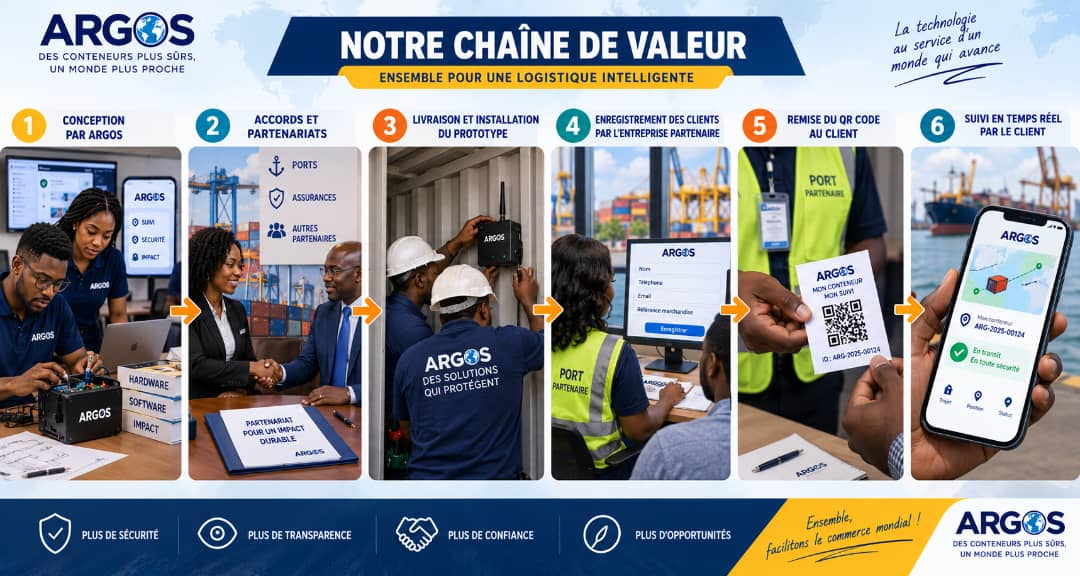
\includegraphics{figures/architecture.jpeg}%
}
\caption{Chaîne de valeur globale et parcours opérationnel ARGOS}
\label{fig-argos-chaine-valeur}
\tablesourcepromoteurs
\end{figure}

Cette architecture visuelle met en lumière les points clés suivants :
\begin{itemize}
    \item \textbf{R\&D et fabrication interne (\textit{Hardware} et \textit{Software}) :} maîtrise initiale de la conception des boîtiers intelligents et des interfaces logicielles par l'équipe technique d'ARGOS.
    \item \textbf{Ancrage partenarial et institutionnel :} formalisation des accords avec les autorités portuaires, les assurances et les acteurs logistiques pour assurer la conformité opérationnelle.
    \item \textbf{Déploiement physique et traçabilité sur le terrain :} installation matérielle autonome des boîtiers connectés à l'intérieur des conteneurs, couplée à un enregistrement rigoureux des profils clients.
    \item \textbf{Sécurisation des accès et supervision en temps réel :} remise d'un identifiant cryptographique unique (QR code) au client final et suivi télématique distant de l'acheminement des marchandises via l'application mobile.
\end{itemize}

En définitive, cette frise valide l'alignement stratégique de la solution autour de quatre piliers fondamentaux : la sécurité matérielle, la transparence des flux, la confiance partenariale et l'optimisation des opportunités logistiques.

\subsubsection{Architecture fonctionnelle}

La figure \ref{fig-architecture-systeme} présente l'architecture fonctionnelle et technique globale du système ARGOS. Ce schéma illustre de manière synthétique l'interaction entre les différentes composantes de la solution, de l'acquisition des données jusqu'à leur restitution.

\begin{figure}[htbp]
    \centering
    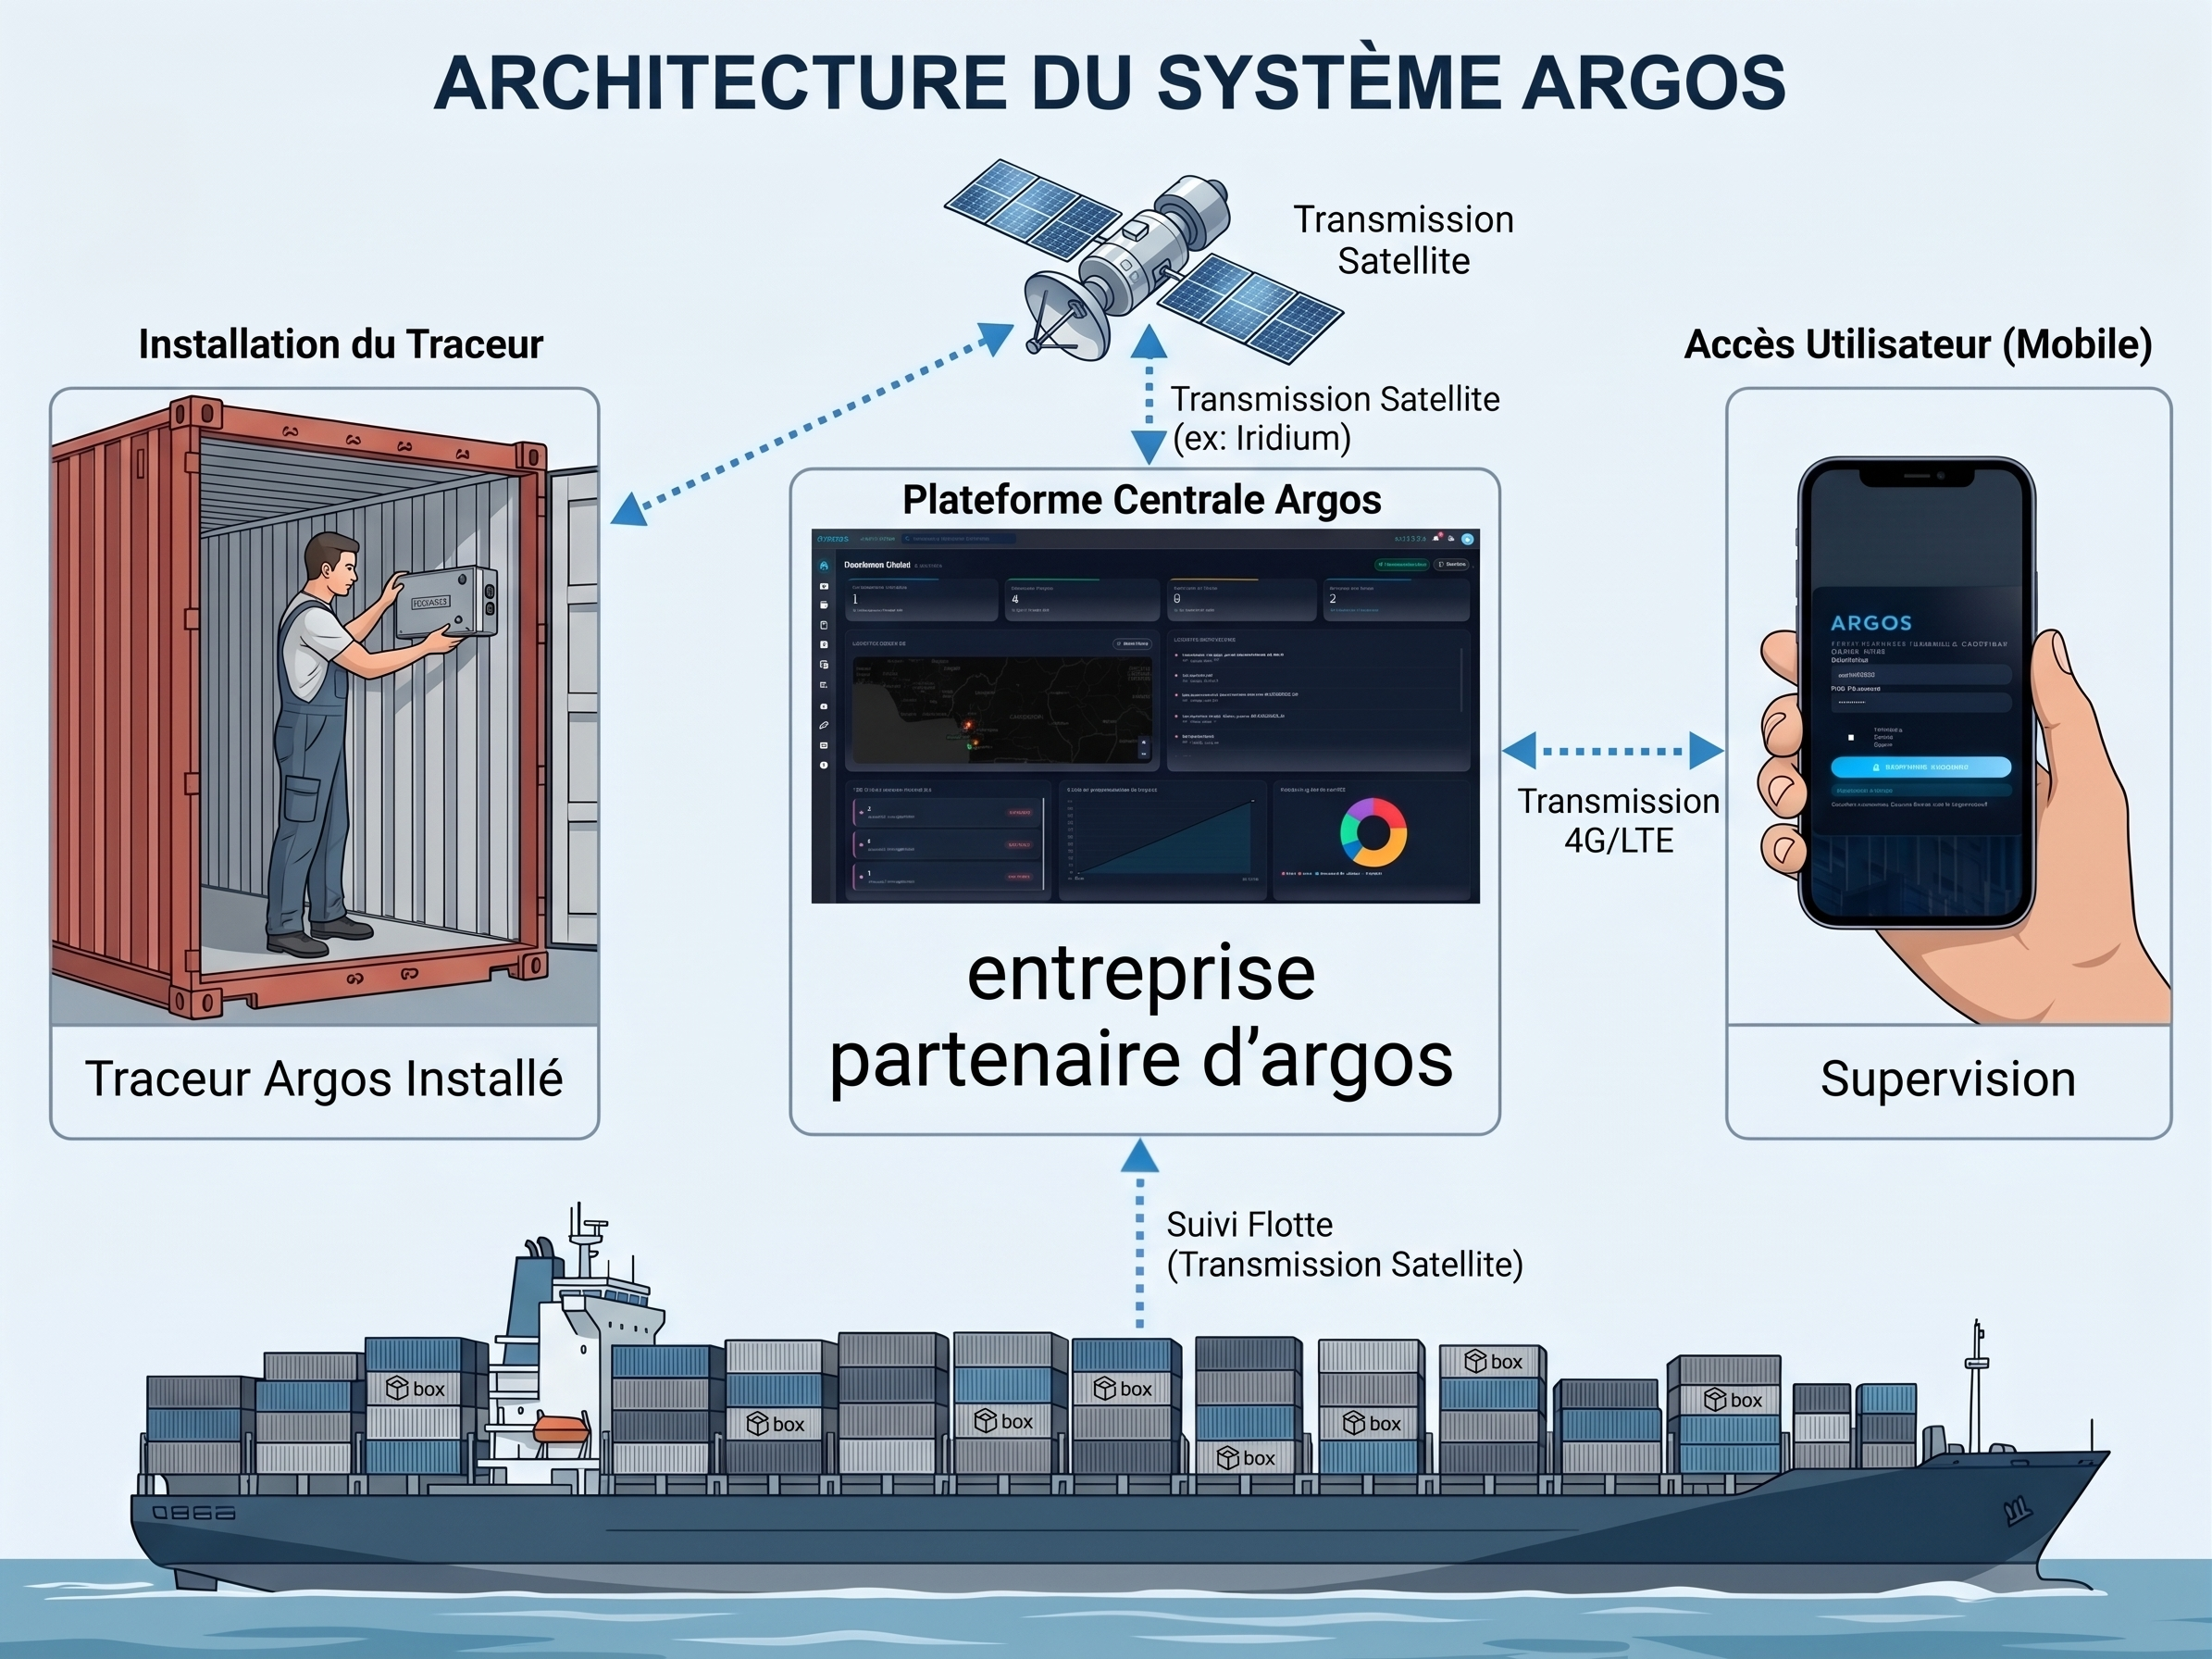
\includegraphics[width=\linewidth,keepaspectratio]{arch.jpeg}
    \caption{Architecture globale et flux de communication du système ARGOS}
    \label{fig-architecture-systeme}
    \tablesourcepromoteurs
\end{figure}

\begin{figure}[htbp]
    \centering
    % Architecture issue du code déployé. Vue volontairement synthétique pour
% rendre visibles les responsabilités et les stockages sans croiser les flux.
\resizebox{\textwidth}{!}{%
\begin{tikzpicture}[
  font=\sffamily\Large,
  client/.style={draw=argosmid,rounded corners=6pt,fill=white,
    text width=8.0cm,minimum height=2.4cm,align=center,line width=1.5pt},
  gateway/.style={draw=argosnavy,rounded corners=6pt,fill=argoslight,
    text width=12.0cm,minimum height=2.8cm,align=center,line width=1.6pt},
  service/.style={draw=argosmid,rounded corners=6pt,fill=argospale,
    text width=8.0cm,minimum height=2.8cm,align=center,line width=1.5pt},
  store/.style={draw=argosnavy,cylinder,shape border rotate=90,aspect=.22,
    fill=white,text width=8.2cm,minimum height=2.9cm,align=center,line width=1.6pt},
  worker/.style={draw=argosnavy,rounded corners=6pt,fill=argoslight,
    text width=8.0cm,minimum height=2.7cm,align=center,line width=1.6pt},
  external/.style={draw=argosrule,rounded corners=6pt,fill=white,
    text width=8.0cm,minimum height=2.4cm,align=center,line width=1.5pt},
  layer/.style={draw=argosrule,rounded corners=8pt,inner sep=10mm,line width=1.5pt},
  title/.style={font=\sffamily\huge\bfseries,text=argosblue,
    fill=white,inner sep=5pt},
  flow/.style={draw=argosgray,line width=1.6pt,-{Stealth[length=4.5mm]}},
  bidir/.style={draw=argosgray,line width=1.6pt,
    {Stealth[length=4.5mm]}-{Stealth[length=4.5mm]}},
  async/.style={draw=argosmid,dashed,line width=1.6pt,-{Stealth[length=4.5mm]}},
  bus/.style={draw=argosgray,line width=1.6pt},
  edgeLabel/.style={font=\sffamily\Large\bfseries,fill=white,inner sep=3pt,align=center}
]

% 1. Canaux d'acquisition.
\node[client] (web) at (-16.0,16.0)
  {Navigateur ARGOS\\Jinja, HTML/CSS et JavaScript};
\node[client] (station) at (0,16.0)
  {ESP32 en mode station\\HTTP REST + \texttt{X-Device-Key}};
\node[client] (ap) at (16.0,16.0)
  {ESP32 en point d'accès\\API locale \texttt{192.168.4.1}};
\node[layer,fit=(web)(station)(ap)] (clients) {};
\node[title] at (0,18.3) {CLIENTS ET CANAUX D'ACQUISITION};

% 2. Façades HTTP et contrôles.
\node[gateway] (webapi) at (-9.5,10.2)
  {Flask / Gunicorn et 12 blueprints\\API métier, Bearer signé, rôle et périmètre};
\node[gateway] (iotapi) at (9.5,10.2)
  {Contrôleurs IoT\\clé technique, enrôlement, télémétrie, audio, commandes et pont direct};
\node[layer,fit=(webapi)(iotapi)] (gateways) {};
\node[title] at (0,12.5) {COUCHE HTTP ET CONTRÔLE D'ACCÈS};

% 3. Services du monolithe.
\node[service] (business) at (-17.5,3.8)
  {Logistique et comptes\\conteneurs, boîtes, BIC, maritime et workflows};
\node[service] (iot) at (-5.8,3.8)
  {Pipeline IoT commun\\validation, liaison, séquence, qualité et seuils};
\node[service] (projection) at (5.8,3.8)
  {Projection applicative\\carte, boîtes, statistiques, alertes et événements};
\node[service] (documents) at (17.5,3.8)
  {Documents et diffusion\\PDF, QR, notifications internes et e-mail};
\node[layer,fit=(business)(iot)(projection)(documents)] (services) {};
\node[title] at (0,6.2) {SERVICES MÉTIER DU MONOLITHE MODULAIRE};

% 4. Données et traitement différé.
\node[store] (postgres) at (-16.5,-3.5)
  {PostgreSQL / TimescaleDB\\schéma \texttt{brady} : métier, mesures, positions, événements, audit et tâches};
\node[worker] (worker) at (-5.5,-3.5)
  {Worker Python\\verrouille \texttt{background\_jobs} dans PostgreSQL};
\node[store] (redis) at (6.0,-3.5)
  {Redis\\DB0 : limitation de débit\\DB1 : \texttt{latest} + stream IoT};
\node[store] (private) at (17.5,-3.5)
  {Volume privé persistant\\audio, contrats, inventaires et rapports};
\node[layer,fit=(postgres)(worker)(redis)(private)] (data) {};
\node[title] at (0,-0.8) {DONNÉES ET TRAITEMENTS DIFFÉRÉS};

% 5. Adaptateurs externes.
\node[external] (providers) at (-17.5,-10.5)
  {BIC BoxTech et fournisseur maritime\\adaptateurs configurables};
\node[external] (transport) at (-5.8,-10.5)
  {Transport de commandes\\HTTP ; MQTT/TLS optionnel};
\node[external] (tunnel) at (5.8,-10.5)
  {Cloudflare Tunnel\\publication HTTPS distante};
\node[external] (mail) at (17.5,-10.5)
  {SMTP / Infobip\\e-mail ; WhatsApp optionnel};
\node[layer,fit=(providers)(transport)(tunnel)(mail)] (externals) {};
\node[title] at (0,-8.0) {SYSTÈMES EXTERNES ET ADAPTATEURS};

% Entrées : le point d'accès est lu par le navigateur, jamais par le VPS.
\draw[flow] (web.south) -- node[edgeLabel,right]{HTTPS / JSON} (webapi.north west);
\draw[flow] (station.south) -- node[edgeLabel,right]{\texttt{/api/iot/*}} (iotapi.north west);
\draw[flow] (ap.south) -- ++(0,-0.85) -| node[edgeLabel,pos=.15,below]{lecture locale HTTP} (web.south east);
\draw[flow] (webapi.east) -- node[edgeLabel,above]{pont direct authentifié} (iotapi.west);

% Les deux façades distribuent vers un bus de services internes.
\draw[flow] (webapi.south) -- (-9.5,5.6);
\draw[flow] (iotapi.south) -- (9.5,5.6);
\draw[bus] (-17.5,5.6) -- (17.5,5.6);
\draw[flow] (-17.5,5.6) -- (business.north);
\draw[flow] (-5.8,5.6) -- (iot.north);
\draw[flow] (5.8,5.6) -- (projection.north);
\draw[flow] (17.5,5.6) -- (documents.north);

% Persistance et temps réel.
\draw[bidir] (business.south) -- node[edgeLabel,right]{métier} (postgres.north west);
\draw[flow] (iot.south west) -- node[edgeLabel,left]{durable} (postgres.north east);
\draw[bidir] (iot.south east) -- node[edgeLabel,left]{cache + stream} (redis.north west);
\draw[bidir] (projection.south) -- node[edgeLabel,right]{Redis d'abord} (redis.north);
\draw[bidir] (documents.south) -- (private.north);
\draw[bidir] (worker.west) -- node[edgeLabel,above]{\texttt{SKIP LOCKED}} (postgres.east);

\node[font=\sffamily\Large,text=argosgray,align=center] at (0,-13.2)
  {Figure~\ref{fig-argos-architecture} : architecture logicielle de la solution ARGOS.};
\end{tikzpicture}%
}
    \caption{Architecture logicielle}
    \label{fig-argos-architecture}
    \tablesourcepromoteurs

\end{figure}

La \cref{fig-argos-architecture} détaille la structure interne d'ARGOS sous la forme d'un monolithe modulaire organisé en cinq couches fonctionnelles superposées. Cette découpe assure une séparation stricte entre les réseaux d'acquisition, le contrôle d'accès, la logique métier, la persistance hybride et les intégrations tierces.

\paragraph{Clients et canaux d'acquisition.}
L'accès à la plateforme s'effectue via trois canaux complémentaires. Le navigateur web charge l'interface dynamique et consomme les API distantes. Sur le terrain, l'ESP32-S3 transmet sa télémétrie au serveur distant en mode station via le protocole HTTP REST sécurisé par la clé \code{X-Device-Key}. En mode point d'accès (\code{192.168.4.1}), le boîtier expose une API locale directement interrogeable par le navigateur client, qui agit alors comme un pont applicatif contrôlé entre le sous-réseau local du matériel et la plateforme ARGOS.

\paragraph{Couche HTTP et contrôle d'accès.}
La façade d'entrée est opérée par Gunicorn exécutant la fabrique d'application Flask, découpée en 12 \emph{blueprints}. Un filtre d'authentification centralisé intercepte l'ensemble des routes sous \code{/api/}, exigeant un jeton Bearer signé ainsi qu'une vérification stricte du rôle et du périmètre de l'utilisateur. En parallèle, les contrôleurs IoT gèrent l'enrôlement, la validation des clés techniques, l'ingestion de la télémétrie, le flux audio, l'émission des commandes et la session du pont direct.

\paragraph{Services métier du monolithe modulaire.}
La logique applicative regroupe quatre domaines fondamentaux à savoir :
\begin{itemize}
    \item \textbf{Logistique et comptes :} gestion du parc de conteneurs, des boîtes noires, intégration des normes BIC/BoxTech, suivi des trajets maritimes et orchestration des workflows ;
    \item \textbf{Pipeline IoT commun :} validation du contrat JSON, contrôle de séquence, évaluation de la qualité des capteurs et calcul automatique du franchissement des seuils d'alerte ;
    \item \textbf{Projection applicative :} agrégation temps réel pour la cartographie, suivi de l'état des boîtes, calcul des indicateurs statistiques et génération des événements ;
    \item \textbf{Documents et diffusion :} création automatique des rapports PDF, génération des QR codes, diffusion des notifications internes et expédition des courriels.
\end{itemize}

\paragraph{Données et traitements différés.}
La persistance repose sur une architecture hybride optimisée :
\begin{itemize}
    \item \textbf{Redis (Multi-DB) :} la base DB0 assure la limitation de débit (\emph{rate limiting}) pour prémunir le serveur contre les dénis de service, tandis que la base DB1 conserve l'instantané de la dernière mesure (\emph{latest}, durée de vie de 24 heures) et le flux tampon (\emph{stream}) borné à environ $10\,000$ entrées pour un affichage dynamique à très faible latence ;
    \item \textbf{PostgreSQL / TimescaleDB (Schéma \code{argos}) :} constitue la source de vérité durable pour l'ensemble des entités métier, lectures de capteurs, positions GPS, événements, journaux d'audit et tâches d'arrière-plan ;
    \item \textbf{Worker Python :} dépile et exécute de façon sécurisée les tâches différées (\code{background\_jobs}) enregistrées en base au moyen du verrouillage SQL \code{SKIP LOCKED} ;
    \item \textbf{Volume privé persistant :} garantit le stockage isolé des fichiers sensibles (segments audio, contrats PDF, inventaires et rapports) hors du répertoire statique public.
\end{itemize}

\paragraph{Systèmes externes et adaptateurs.}
La couche inférieure regroupe les connecteurs d'intégration : les adaptateurs BIC BoxTech et maritimes pour la normalisation du suivi, le transport HTTP/MQTT pour l'exécution distante des commandes, l'exposition distante sécurisée via Cloudflare Tunnel (HTTPS/HTTP2) sans ouverture directe des ports du routeur, ainsi que les passerelles SMTP et Infobip pour la diffusion des alerteurs par courriel ou WhatsApp.

\subsubsection{Organisation des modules}

\begin{longtable}{@{}p{3.2cm}p{5.6cm}p{6.2cm}@{}}
\caption{Organisation des douze blueprints Flask}
\label{tab-blueprints-argos}\\
\tableheadrow \thc{Blueprint} & \thc{Routes principales} & \thc{Responsabilités} \\
\midrule
\endfirsthead
\tableheadrow \thc{Blueprint} & \thc{Routes principales} & \thc{Responsabilités} \\
\midrule
\endhead
\code{auth} & \code{/api/login}, \code{/api/auth/*} & Connexion, disponibilité du login et changement du mot de passe \\
\hline
\code{dashboard} & \code{/}, \code{/api/stats*}, \code{/api/dashboard/*} & Page principale, KPI, statistiques historiques et temps réel \\
\hline
\code{containers} & \code{/api/containers/*}, \code{/api/notifications} & Parc de conteneurs, positions, vente, inventaire et notification \\
\hline
\code{black\_boxes} & \code{/api/black-boxes/*} & Création, QR, affectation, reconnexion, session directe, rapport et archivage \\
\hline
\code{boites\_noires} & \code{/api/boites-noires/*}, \code{/api/captive/*} & Compatibilité historique et parcours du portail captif \\
\hline
\code{telemetry} & \code{/api/telemetry}, \code{/api/config/thresholds}, \code{/api/events} & Compatibilité de télémétrie, seuils, monitoring et événements \\
\hline
\code{iot} & \code{/api/iot/*}, \code{/api/black-boxes/*/commands/*} & Enrôlement, ingestion, audio, commandes, acquittements et mode sécurité \\
\hline
\code{users} & \code{/api/companies}, \code{/api/clients}, \code{/api/drivers} & Comptes, entreprises, clients, chauffeurs et abonnements \\
\hline
\code{workflows} & \code{/api/contracts/*}, \code{/api/documents}, \code{/api/destocking/*} & Contrats, inventaires, documents, vote et déstockage \\
\hline
\code{maritime} & \code{/api/container/validate}, \code{/api/voyage/*}, \code{/api/litiges} & BIC, voyages, tracking et contrôles portuaires \\
\hline
\code{blockchain} & \code{/api/blockchain/*} & Consultation, statistiques et vérification du journal d'événements \\
\hline
\code{publication} & \code{/api/publications} & Création et consultation des publications \\
\tablebottomrule
\end{longtable}
\tablesourcepromoteurs

\subsection{Organigramme de l'application}

\begin{figure}[H]
    \centering
    \resizebox{\textwidth}{!}{% Force le schéma à tenir dans la largeur de la page
        \resizebox{\textwidth}{!}{%
\begin{tikzpicture}[
  font=\sffamily\small,
  start/.style={draw=argosnavy,rounded corners=8pt,fill=argoslight,
    text width=4.8cm,minimum height=1.3cm,align=center,line width=1pt},
  action/.style={draw=argosmid,rounded corners=4pt,fill=white,
    text width=4.8cm,minimum height=1.3cm,align=center,line width=.9pt},
  decision/.style={draw=argosnavy,diamond,aspect=2.2,fill=argospale,
    text width=3.4cm,minimum height=1.6cm,align=center,line width=1pt},
  module/.style={draw=argosrule,rounded corners=4pt,fill=argospale,
    text width=3.8cm,minimum height=1.4cm,align=center,line width=.9pt},
  api/.style={draw=argosblue,rounded corners=4pt,fill=argoslight,
    text width=6.5cm,minimum height=1.3cm,align=center,line width=1pt},
  flow/.style={draw=argosgray,line width=1pt,-{Stealth[length=3mm]}},
  label/.style={font=\sffamily\scriptsize\bfseries,fill=white,inner sep=2pt}
]

% 1. Authentification & Connexion
\node[start] (open) at (0,12.0) {Ouverture de l'application ARGOS};
\node[decision] (token) at (0,9.5) {Jeton signé valide ?};
\node[action] (login) at (-7.5,9.5) {Saisir le login et le mot de passe};
\node[decision] (credentials) at (-7.5,6.8) {Identifiants valides ?};
\node[action] (reject) at (-13.5,6.8) {Refus, message d'erreur};

% 2. Validation & Chargement du Périmètre
\node[decision] (contract) at (0,6.8) {Contrat en attente ?};
\node[action] (accept) at (-6.8,3.8) {Lire, télécharger et décider};
\node[action] (scope) at (0,3.8) {Charger le rôle et le périmètre\\de ressources autorisées};
\node[action] (nav) at (0,1.0) {Construire le menu du profil\\et ouvrir le tableau de bord};

% Flux d'authentification
\draw[flow] (open) -- (token);
\draw[flow] (token.west) -- node[label,above]{non} (login.east);
\draw[flow] (login) -- (credentials);
\draw[flow] (credentials.west) -- node[label,above]{non} (reject.east);
\draw[flow] (reject.north) |- (login.west);
\draw[flow] (credentials.east) -- node[label,above]{oui} (contract.west);
\draw[flow] (token) -- node[label,right]{oui} (contract);
\draw[flow] (contract.south west) -- node[label,above,sloped]{oui} (accept.north east);
\draw[flow] (accept.east) -- node[label,above]{accepté} (scope.west);
\draw[flow] (contract) -- node[label,right]{non} (scope);
\draw[flow] (scope) -- (nav);

% 3. Modules Applicatifs (Espacement horizontal de 4.4cm)
\node[module] (dash) at (-11.0,-2.0) {Tableau de bord\\KPI et état du parc};
\node[module] (map) at (-6.6,-2.0) {Carte et conteneurs\\positions, trajets, détails};
\node[module] (boxes) at (-2.2,-2.0) {Boîtes noires\\QR, affectation, connexion};
\node[module] (stats) at (2.2,-2.0) {Statistiques\\filtres et séries temporelles};
\node[module] (events) at (6.6,-2.0) {Événements et alertes\\tri, lecture, notifications};
\node[module] (docs) at (11.0,-2.0) {Documents et workflows\\contrats, inventaire, déstockage};

\foreach \target in {dash,map,boxes,stats,events,docs}
  \draw[flow] (nav.south) -- ++(0,-1.0) -| (\target.north);

% 4. Contrôle de Rôle & Actions Métier
\node[decision] (manager) at (-5.0,-5.2) {Gestionnaire autorisé ?};
\node[action] (direct) at (-10.5,-8.2) {Mode direct : vérifier \texttt{deviceUid},\\lire l'AP et synchroniser la file};
\node[action] (security) at (-5.0,-8.2) {Activer ou bloquer la sécurité\\et auditer l'auteur};
\node[action] (consult) at (3.5,-8.2) {Consultation filtrée selon\\rôle, boîte et conteneur};

% Flux métiers
\draw[flow] (boxes.south) |- (manager.north);
\draw[flow] (manager.south west) -- node[label,above,sloped]{oui} (direct.north east);
\draw[flow] (manager) -- node[label,right]{oui} (security);
\draw[flow] (map.south) |- (consult.north);
\draw[flow] (stats.south) |- (consult.north);
\draw[flow] (events.south) |- (consult.north);
\draw[flow] (docs.south) |- (consult.north);
\draw[flow] (manager.east) -- node[label,above]{non} (consult.west);

% 5. API Backend & Rendu Final
\node[api] (api) at (0,-11.2) {Appel API avec jeton Bearer\\contrôle rôle + propriété de la ressource};
\node[action] (data) at (0,-13.8) {Lecture Redis temps réel ou PostgreSQL\\puis rendu carte, boîtes, statistiques et événements};

\draw[flow] (direct.south) |- (api.west);
\draw[flow] (security.south) -- (api.north west);
\draw[flow] (consult.south) -- (api.north east);
\draw[flow] (api) -- (data);

\end{tikzpicture}%
}
    }
    \caption{Organigramme fonctionnel de navigation et de contrôle d'accès}
    \label{fig-argos-organigramme-application}
    \tablesourcepromoteurs
\end{figure}

L'organigramme de la \cref{fig-argos-organigramme-application} montre que le
menu n'est pas une preuve d'autorisation. Il améliore l'ergonomie en masquant
les pages étrangères au rôle, tandis que les principales API privées
recalculent le périmètre des boîtes et conteneurs autorisés. Le
superadministrateur reçoit le périmètre
global ; les autres profils reçoivent une liste issue des liens de propriété,
d'agence, d'abonnement, de transport ou de port.

\section{Conception détaillée}

Cette section approfondit les choix de conception présentés précédemment en entrant dans le détail technique de leur mise en œuvre. Elle décrit notamment l'architecture matérielle du prototype, les mécanismes de sécurité mis en place ainsi que la modélisation du système à travers différents diagrammes. Elle a pour but de montrer concrètement comment les orientations générales du projet se traduisent en solutions techniques précises et réalisables.

\subsection{Architecture du prototype ESP32}

L'ESP32 est un microcontrôleur à faible consommation d'énergie, doté d'une connectivité Wi-Fi et Bluetooth intégrée, largement utilisé dans les projets d'objets connectés (IoT). Il permet de piloter divers capteurs et modules de communication tout en assurant le traitement local des données. Cette section présente l'architecture du prototype ARGOS construite autour de ce composant, en détaillant le raccordement matériel des différents éléments ainsi que le fonctionnement du micrologiciel qui les pilote.

\subsubsection{Raccordement matériel}

Cette section décrit la manière dont les différents composants électroniques du prototype ARGOS sont physiquement reliés au microcontrôleur ESP32. Elle précise pour chaque élément capteurs, module de communication, module GPS, carte mémoire, alarme et indicateurs lumineux la broche à laquelle il est connecté ainsi que la fonction qu'il assure. Cette présentation permet de comprendre l'organisation matérielle du dispositif avant d'aborder le fonctionnement logiciel qui l'exploite.

\begin{table}[htbp]
\centering
\caption{Affectation des broches du micrologiciel ARGOS}
\label{tab-broches-esp32}
\begin{tabularx}{\textwidth}{@{}p{3.5cm}p{2.2cm}X@{}}
\tableheadrow \thc{Élément} & \thc{GPIO} & \thc{Fonction} \\
\midrule
LED bleue & 1 & Témoin d'alimentation et de fonctionnement, maintenu allumé en permanence \\
\hline
Bouton BOOT & 0 & Appui de trois secondes pour revenir au mode de configuration \\
\hline
Photorésistance LDR & 3 & Niveau lumineux et contribution à la détection d'ouverture \\
\hline
AM2302/DHT22 & 4 & Température et humidité \\
\hline
Microphone analogique & 5 & Niveau sonore \\
\hline
HC-SR04 & 6 / 7 & Déclenchement et écho de la mesure de distance \\
\hline
MPU6050 & 8 / 9 & Bus I\textsuperscript{2}C SDA/SCL, accélérations et choc \\
\hline
Buzzer & 10 & Alarme locale \\
\hline
Carte microSD & 11 / 12 / 13 / 14 & SPI MOSI, SCK, MISO et CS pour le journal local \\
\hline
SIM800 & 15 / 16 & UART prévu pour la communication cellulaire \\
\hline
GPS NEO-6M & 17 / 18 & UART de localisation \\
\hline
Capteur de flamme & 21 & Détection numérique de flamme \\
\hline
LED RGB intégrée & 48 par défaut & État visuel complémentaire de la carte ESP32-S3 \\
\tablebottomrule
\end{tabularx}
\tablesourcepromoteurs
\end{table}

\subsubsection{Cycle de vie du micrologiciel}

Au démarrage, le micrologiciel initialise les entrées/sorties, teste les LED,
interroge le DHT22, le MPU6050 et la carte SD, puis charge les paramètres
conservés dans \code{Preferences}. Le \code{deviceUid} est dérivé de l'eFuse
si aucune identité n'existe encore. Les numéros de séquence sont réservés par
blocs de 64 afin de rester monotones après un redémarrage sans user la mémoire
flash à chaque mesure.

Si le Wi-Fi, l'URL d'API ou l'identité de boîte manquent, ou après trois
échecs de connexion, l'ESP32 crée le réseau
\code{ARGOS-SETUP-...}. Son serveur local expose :
\begin{itemize}
    \item \code{GET /api/device/info} pour l'identité et les modes ;
    \item \code{GET /api/v1/telemetry} pour le dernier instantané ;
    \item \code{POST /api/v1/security} pour le mode de sécurité local ;
    \item \code{POST /api/v1/provision} pour recevoir la configuration ;
    \item \code{POST /api/v1/register} pour le parcours captif historique.
\end{itemize}

En mode station, l'appareil s'enrôle si sa clé permanente est absente, vérifie
les commandes toutes les cinq secondes et transmet normalement une mesure
toutes les trente secondes. Une nouvelle alarme provoque un envoi anticipé.
Le buzzer dépend du mode sécurité, de la distance, des seuils locaux et de la
détection de flamme. Le mode porte est initialement bloqué et ne peut être
activé que par un gestionnaire autorisé dans l'application.

\subsection{Sécurité et restrictions d'accès}

Cette section présente les mécanismes mis en place pour protéger l'accès à la plateforme ARGOS et contrôler les actions que peut effectuer chaque utilisateur. Elle aborde successivement l'authentification des utilisateurs, la gestion des jetons de session et les règles qui déterminent les droits accordés selon le profil. L'objectif est de garantir que seules les personnes autorisées puissent consulter ou modifier les données sensibles du système.

\subsubsection{Authentification humaine}

Après vérification du hash Werkzeug du mot de passe, ARGOS émet un jeton
Bearer signé et horodaté au moyen de
\code{itsdangerous.URLSafeTimedSerializer}. Il ne s'agit pas d'un JWT. Sa
durée maximale est de 28\,800 secondes par défaut. Il contient le rôle,
l'identifiant, le login, le nom affiché, la portée et la
\code{token\_version}. Le registre \code{identity\_registry} garantit
l'unicité du login entre les familles de comptes et permet de révoquer les
sessions après un changement de mot de passe ou une désactivation.

Les en-têtes historiques \code{X-Role} et \code{X-User-Id} sont ignorés comme
preuves d'identité. Un compte dont le contrat est en attente reçoit une portée
limitée aux routes de consultation et de décision du contrat.

\subsubsection{Authentification du dispositif}

Le provisionnement crée un \code{deviceUid}, un jeton d'enrôlement temporaire
et l'association à une boîte. Seule l'empreinte du jeton est conservée.
L'enrôlement retourne une clé permanente affichée une seule fois ; son hash
est stocké dans \code{iot\_devices}. Une télémétrie distante n'est acceptée
que si la clé, l'état \code{ACTIVE}, la boîte, le conteneur et la séquence
correspondent.

En mode direct, la clé permanente n'est jamais remise au navigateur. Le
navigateur présente son jeton humain au serveur et ARGOS exige l'égalité
exacte entre l'UID lu sur \code{192.168.4.1} et celui associé à la boîte.

\subsubsection{Matrice synthétique des autorisations}

\begin{table}[htbp]
\centering
\small
\caption{Droits fonctionnels principaux par profil}
\label{tab-matrice-roles}
\begin{tabularx}{\textwidth}{@{}p{3.0cm}*{6}{>{\centering\arraybackslash}X}@{}}
\tableheadrow \thc{Fonction} & \thc{Super-admin} & \thc{Proprié-taire} & \thc{Entreprise} & \thc{Client} & \thc{Transpor-teur} & \thc{Autorité portuaire} \\
\midrule
Voir le parc autorisé & Global & Propre & Délégué & Abonné & Mission & Port \\
\hline
Créer/affecter une boîte & Oui & Propre parc & Non & Non & Non & Non \\
\hline
Connexion directe ESP32 & Oui & Propre parc & Déléguée & Non & Non & Non \\
\hline
Activer/bloquer la sécurité & Oui & Propre parc & Déléguée & Non & Non & Non \\
\hline
Statistiques et événements & Global & Propre parc & Délégués & Liés & Liés & Port \\
\hline
Gérer comptes et abonnements & Oui & Clients et chauffeurs liés & Clients liés & Non & Non & Non \\
\hline
Contrôle maritime et douanier & Oui & Consult. & Consult. & Consult. liée & Consult. liée & Oui \\
\tablebottomrule
\end{tabularx}
\tablesourcepromoteurs
\end{table}

\subsection{Diagramme de classes}

Le diagramme de la \cref{fig-argos-classes} expose la vue conceptuelle des entités métiers qui composent la plateforme ARGOS. Cette modélisation UML s'attache à traduire la logique métier du système indépendamment de sa mise en œuvre logicielle, l'implémentation effective s'appuyant sur des services applicatifs et des requêtes SQL optimisées.

La conception statique de la plateforme repose sur un principe fondamental de découplage entre le conteneur logistique, la boîte noire logicielle et le dispositif matériel (ESP32). Cette séparation garantit une grande flexibilité opérationnelle : la réaffectation d'une boîte noire à un nouveau conteneur ou le remplacement d'un composant électronique défectueux s'effectuent sans discontinuité et sans altération de la traçabilité historique des mesures.

Afin d'assurer la cohérence globale des données et de faciliter la maintenance de l'application, le domaine métier est structuré autour de quatre agrégats majeurs :

\begin{itemize}
    \item \textbf{Agrégat 1 : Identités et Organisations :} Il constitue le socle de la gestion des accès et de la confidentialité. Cet agrégat regroupe la définition des profils utilisateurs, la résolution centralisée des rôles applicatifs et la délimitation stricte du périmètre de visibilité des parties prenantes sur les ressources du parc.
    
    \item \textbf{Agrégat 2 : Logistique et Workflows :} Il orchestre l'ensemble du cycle de vie opérationnel. Il régit la traçabilité des conteneurs, le suivi temporel des affectations de boîtes noires et la gouvernance des processus métiers complexes, notamment les procédures collaboratives de déstockage.
    
    \item \textbf{Agrégat 3 : Dispositifs et Télémétrie :} Il encadre la chaîne d'acquisition de données issues du terrain. Cet agrégat assure l'identification unique du matériel embarqué, la réception des messages bruts ainsi que leur transformation en observations physiques qualifiées (température, humidité, chocs) et en coordonnées de géolocalisation.
    
    \item \textbf{Agrégat 4 : Exploitation et Audit :} Il garantit la réactivité du système et l'immuabilité de la preuve. Il prend en charge la détection d'anomalies, la diffusion ciblée des alertes, le scellement de sécurité des événements critiques et la journalisation systématique des actions d'exploitation.
\end{itemize}

La correspondance détaillée entre ces concepts fonctionnels et la structure des tables physiques actuellement déployées en base de données est synthétisée dans le \cref{tab-correspondance-classes}.

\begin{table}[htbp]
\centering
\small
\caption{Correspondance entre agrégats métiers et tables de la base de données}
\label{tab-correspondance-classes}
\begin{tabularx}{\textwidth}{@{}p{4.0cm}p{5.0cm}X@{}}
\tableheadrow \thc{Agrégat} & \thc{Tables centrales} & \thc{Portée fonctionnelle} \\
\midrule
Identités \& Organisations & \code{identity\_registry}, tables de profils & Authentification, contrôle d'accès basé sur les rôles et périmètres de visibilité. \\
\hline
Logistique \& Workflows & \code{conteneurs}, \code{boite\_noir}, \code{assignments}, \code{destocking\_requests} & Gestion du parc, traçabilité des liaisons et suivi des processus d'approbation. \\
\hline
Dispositifs \& Télémétrie & \code{iot\_devices}, \code{iot\_raw\_messages}, \code{sensor\_readings}, \code{positions} & Registre du matériel, ingestion des paquets bruts et persistance des séries temporelles. \\
\hline
Exploitation \& Audit & \code{evenement\_save}, \code{notifications}, \code{audit\_logs}, \code{blockchain\_argos} & Traitement des alertes, traçabilité des opérations et scellement d'intégrité. \\
\tablebottomrule
\end{tabularx}
\tablesourcepromoteurs
\end{table}

\begin{figure}[htbp]
\centering
\resizebox{0.95\textwidth}{!}{%
  % Diagramme de classes métier ARGOS — Version aérée et lisible
\resizebox{\textwidth}{!}{%
\begin{tikzpicture}[
  font=\sffamily\small,
  uml/.style={draw=argosnavy,line width=1.1pt,rectangle split,
    rectangle split parts=2,align=left,inner sep=6pt,text width=5.0cm,fill=white},
  group/.style={draw=argosrule,dashed,rounded corners=6pt,inner sep=8mm,line width=1.2pt},
  assoc/.style={draw=argosgray,line width=1.1pt},
  dep/.style={draw=argosgray,dashed,line width=1.1pt,-{Stealth[length=3mm]}},
  mult/.style={font=\sffamily\small\bfseries,fill=white,inner sep=2pt},
  title/.style={font=\sffamily\large\bfseries,text=argosblue,fill=white,inner sep=4pt}
]

% ==========================================
% AGRÉGAT 1 — IDENTITÉS ET ORGANISATIONS
% ==========================================
\node[uml] (profile) at (-12,13) {\textbf{ProfilActeur}
  \nodepart{second}\texttt{idActeur : String}\\\texttt{rôle : Rôle}\\\texttt{login : String}};

\node[uml] (identity) at (-4,13) {\textbf{Identité}
  \nodepart{second}\texttt{actorRole : String}\\\texttt{actorId : String}\\\texttt{displayName : String}};

\node[uml] (party) at (4,13) {\textbf{PartieLogistique}
  \nodepart{second}\texttt{type : RôleMetier}\\\texttt{périmètre : List<Boîte>}};

\node[group,fit=(profile)(identity)(party),label={[title]above:AGRÉGAT 1 — IDENTITÉS ET ORGANISATIONS}] {};

\draw[assoc] (profile) -- node[mult,near start,above]{1} node[mult,near end,above]{1} (identity);
\draw[dep] (identity) -- node[mult,above]{résout} (party);


% ==========================================
% AGRÉGAT 2 — LOGISTIQUE ET WORKFLOWS
% ==========================================
\node[uml] (container) at (-12,6.5) {\textbf{Conteneur}
  \nodepart{second}\texttt{idConteneur : String}\\\texttt{type, statut : String}};

\node[uml] (box) at (-4,6.5) {\textbf{BoîteNoire}
  \nodepart{second}\texttt{idBoîte : Integer}\\\texttt{uuidQr : UUID}\\\texttt{statut : Boolean}};

\node[uml] (assignment) at (4,6.5) {\textbf{AffectationBoîteConteneur}
  \nodepart{second}\texttt{assignedAt : DateTime}\\\texttt{detachedAt : DateTime?}};

\node[uml] (destock) at (12,6.5) {\textbf{DemandeDéstockage}
  \nodepart{second}\texttt{requiredApprovals : Int}\\\texttt{statut : String}};

\node[group,fit=(container)(box)(assignment)(destock),
  label={[title]above:AGRÉGAT 2 — LOGISTIQUE ET WORKFLOWS}] {};

\draw[assoc] (container) -- node[mult,near start,above]{1} node[mult,near end,above]{0..1} (box);
\draw[assoc] (box) -- node[mult,near start,above]{1} node[mult,near end,above]{0..*} (assignment);
\draw[assoc] (container) |- ++(0,-2.2) -| node[mult,near end,below]{0..*} (destock);


% ==========================================
% AGRÉGAT 3 — DISPOSITIFS ET TÉLÉMÉTRIE
% ==========================================
\node[uml] (device) at (-12,0) {\textbf{DispositifIoT}
  \nodepart{second}\texttt{deviceUid : String}\\\texttt{statut : String}};

\node[uml] (raw) at (-4,0) {\textbf{MessageBrut}
  \nodepart{second}\texttt{messageId : UUID}\\\texttt{payload : JSON}};

\node[uml] (reading) at (4,0) {\textbf{LectureCapteur}
  \nodepart{second}\texttt{sequence : Integer}\\\texttt{temp, humid, choc}};

\node[uml] (position) at (12,0) {\textbf{Position}
  \nodepart{second}\texttt{latitude, longitude}\\\texttt{measuredAt : DateTime}};

\node[group,fit=(device)(raw)(reading)(position),
  label={[title]above:AGRÉGAT 3 — DISPOSITIFS ET TÉLÉMÉTRIE}] {};

\draw[assoc] (device) -- node[mult,near start,above]{1} node[mult,near end,above]{0..*} (raw);
\draw[assoc] (raw) -- node[mult,near start,above]{1} node[mult,near end,above]{0..1} (reading);
\draw[assoc] (raw) |- ++(0,-2.2) -| node[mult,near end,below]{0..1} (position);


% ==========================================
% AGRÉGAT 4 — EXPLOITATION ET AUDIT
% ==========================================
\node[uml] (event) at (-12,-6.5) {\textbf{Événement}
  \nodepart{second}\texttt{idEventInit : BigInt}\\\texttt{horodatage : DateTime}};

\node[uml] (notification) at (-4,-6.5) {\textbf{Notification}
  \nodepart{second}\texttt{type, message : String}\\\texttt{statut : String}};

\node[uml] (audit) at (4,-6.5) {\textbf{JournalAudit}
  \nodepart{second}\texttt{action, entityType}\\\texttt{createdAt : DateTime}};

\node[uml] (block) at (12,-6.5) {\textbf{BlocScellé}
  \nodepart{second}\texttt{blockHash : String}\\\texttt{eventType : String}};

\node[group,fit=(event)(notification)(audit)(block),
  label={[title]above:AGRÉGAT 4 — EXPLOITATION, AUDIT ET PREUVE}] {};

\draw[dep] (event) -- node[mult,above]{alerte} (notification);
\draw[dep] (event) |- ++(0,-2.2) -| node[mult,below]{scellement} (block);


% ==========================================
% LIAISONS ET INTER-RACCORDEMENTS INTER-AGRÉGATS
% ==========================================
% Lien Identité -> Logistique
\draw[assoc] (party.south) |- ++(0,-1.5) -| node[mult,near end,left]{1..*} (container.north);

% Lien BoîteNoire -> Événement
\draw[assoc] (box.south) -- node[mult,near start,right]{1} node[mult,near end,right]{0..*} (event.north);

% Lien DispositifIoT -> JournalAudit
\draw[dep] (device.south) |- ++(0,-1.5) -| node[mult,near end,right]{audit technique} (audit.north);

\end{tikzpicture}%
}%
}
\caption{Diagramme de classes d'ARGOS}
\label{fig-argos-classes}
\end{figure}
\tablesourcepromoteurs

La lecture directe du diagramme de classes permet de formaliser les règles de gestion fondamentales qui régissent les interactions entre les différents agrégats du système ARGOS :

\paragraph{Agrégat « Identités et Organisations »}
La gouvernance des accès repose sur un couplage strict entre les structures d'authentification et les profils. Ainsi, chaque \texttt{ProfilActeur} possède univoquement \textbf{une et une seule} \texttt{Identité}, laquelle se résout et s'articule directement vers une \texttt{PartieLogistique} par le biais d'une relation de dépendance garantissant la portée des droits.

\paragraph{Agrégat « Logistique et Workflows »}
Le suivi du parc opérationnel est conçu pour être flexible et traçable : un \texttt{Conteneur} peut être équipé d'au maximum \textbf{une} \texttt{BoîteNoire} (ou n'en avoir aucune à un instant donné). Pour assurer la traçabilité historique, chaque \texttt{BoîteNoire} fait l'objet de \textbf{zéro à plusieurs} enregistrements d'affectation (\texttt{AffectationBoîteConteneur}), tandis qu'un \texttt{Conteneur} peut initier et concerner \textbf{plusieurs} processus décisionnels de \texttt{DemandeDéstockage}.

\paragraph{Agrégat « Dispositifs et Télémétrie »}
La chaîne d'acquisition de données s'organise autour d'un flux maîtrisé où chaque \texttt{DispositifIoT} génère continuellement des paquets de type \texttt{MessageBrut}. Chacun de ces messages encapsule à son tour au plus \textbf{une} \texttt{LectureCapteur} qualifiée et \textbf{une} \texttt{Position} géolocalisée.

\paragraph{Agrégat « Exploitation, Audit et Preuve »}
La sécurité et la réactivité du système s'appuient sur des mécanismes de traçabilité événementielle. Par des relations de dépendance ciblées, chaque \texttt{Événement} critique déclenche instantanément une alerte sous forme de \texttt{Notification} et implique un scellement immuable au sein d'un \texttt{BlocScellé}.

\paragraph{Liaisons transversales et inter-agrégats}
Enfin, la cohérence globale de l'écosystème est assurée par des ponts relationnels majeurs : toute \texttt{PartieLogistique} doit piloter et gérer \textbf{au moins un} \texttt{Conteneur}. De son côté, chaque \texttt{BoîteNoire} consigne l'ensemble des anomalies sous forme de \textbf{zéro à plusieurs} \texttt{Événement}s, tandis que chaque \texttt{DispositifIoT} documente rigoureusement son intégrité opérationnelle en traçant son audit technique vers le \texttt{JournalAudit}.


\subsection{Diagramme des cas d'utilisation}
\par La modélisation fonctionnelle du diagramme de cas d'utilisation a pour objectif fondamental de décrire le système du point de vue de ses utilisateurs et des acteurs externes avec lesquels il interagit, en mettant en lumière les services et les fonctionnalités offerts par la plateforme. Pour ce faire, le diagramme de cas d'utilisation UML constitue l'outil de référence : son rôle est d'identifier de manière exhaustive les frontières du système ARGOS, de cartographier les interactions entre chaque profil d'utilisateur (humain ou technique) et de formaliser les exigences comportementales attendues. Afin de restituer fidèlement la complexité opérationnelle et administrative du projet, l'analyse fonctionnelle se décline ci-après à travers deux axes complémentaires : d'une part, les cas d'utilisation administratifs, qui régissent la gouvernance et la gestion du parc, et d'autre part, les cas d'utilisation opérationnels, qui encadrent l'exécution sur le terrain et le suivi télématique.

\subsubsection{Cas d'utilisation administratifs}

La modélisation fonctionnelle d'ARGOS s'articule autour de deux vues complémentaires : d'une part, 
les cas d'utilisation administratifs qui régissent la gouvernance, la configuration du parc et la gestion des comptes ; 
d'autre part, les cas d'utilisation opérationnels qui décrivent l'exécution sur le terrain, 
le suivi télématique direct et les interactions avec les dispositifs embarqués.

\begin{figure}[htbp]
\centering
\begin{minipage}{\textwidth}
\centering
\resizebox{0.82\textwidth}{!}{%
  % Diagramme de cas d'utilisation administratifs — ARGOS (Optimisé & Complet)
\resizebox{\textwidth}{!}{%
\begin{tikzpicture}[
  font=\sffamily\large\bfseries,
  uc/.style={draw=argosmid,ellipse,align=center,text width=5.5cm,
    minimum width=6.0cm,minimum height=1.5cm,fill=white,line width=1.4pt},
  link/.style={draw=argosgray,line width=1.4pt},
  inherit/.style={draw=argosnavy,line width=1.4pt,-{Triangle[open,length=4.5mm]}},
  boundary/.style={draw=argosnavy,rounded corners=8pt,inner sep=10mm,line width=1.8pt},
  actorfont/.style={font=\sffamily\large\bfseries,align=center,text=argosnavy}
]

% -----------------------------------------------------------------
% COMMANDE TIKZ POUR DESSINER UN BONSHOMME UML
% -----------------------------------------------------------------
\newcommand{\drawstickman}[3]{ % #1: name, #2: (x,y), #3: label
  \coordinate (center) at #2;
  \draw[draw=argosnavy,line width=1.5pt,fill=argospale] ($(center)+(0,0.9)$) circle (0.42cm);
  \draw[draw=argosnavy,line width=1.5pt] ($(center)+(0,0.48)$) -- ($(center)+(0,-0.4)$);
  \draw[draw=argosnavy,line width=1.5pt] ($(center)+(-0.5,0.25)$) -- ($(center)+(0.5,0.25)$);
  \draw[draw=argosnavy,line width=1.5pt] ($(center)+(0,-0.4)$) -- ($(center)+(-0.4,-1.0)$);
  \draw[draw=argosnavy,line width=1.5pt] ($(center)+(0,-0.4)$) -- ($(center)+(0.4,-1.0)$);
  \node[actorfont,anchor=north] at ($(center)+(0,-1.15)$) {#3};
  \node[rectangle,inner sep=2pt,minimum width=4.0cm,minimum height=3.0cm] (#1) at ($(center)+(0,0.1)$) {};
}

% -----------------------------------------------------------------
% POSITIONNEMENT DES ACTEURS (Echelle Y compacte pour affichage complet)
% -----------------------------------------------------------------
% Acteur racine
\drawstickman{user}{(-15.0, 1.8)}{Utilisateur Authentifié};

% Acteurs intermédiaires
\drawstickman{company}{(-7.5, 5.5)}{Agence / Entreprise};
\drawstickman{port}{(-7.5, -2.0)}{Autorité Portuaire};

% Acteur spécialisé
\drawstickman{owner}{(-15.0, 9.2)}{Propriétaire};

% Acteur suprême
\drawstickman{admin}{(-15.0, 13.5)}{Superadministrateur};

% -----------------------------------------------------------------
% LIENS D'HÉRITAGE (Sur les bordures externes)
% -----------------------------------------------------------------
\draw[inherit] (company.north west) -- node[above,font=\small\bfseries,sloped]{hérite} (user.north east);
\draw[inherit] (port.north west) -- node[below,font=\small\bfseries,sloped]{hérite} (user.south east);
\draw[inherit] (owner.south) -- node[right,font=\small\bfseries]{hérite} (company.north west);
\draw[inherit] (admin.south) -- node[right,font=\small\bfseries]{hérite} (owner.north);

% -----------------------------------------------------------------
% CAS D'UTILISATION (Disposition en grille verticale équilibrée)
% -----------------------------------------------------------------
% Superadministrateur
\node[uc] (accounts) at (4.0, 13.5) {Gérer entreprises, comptes et rôles globaux};
\node[uc] (audit) at (4.0, 11.2) {Consulter et vérifier les données scellées};

% Propriétaire
\node[uc] (fleet) at (4.0, 9.0) {Administrer le parc, boîtes et enrôlement ESP32};
\node[uc] (users) at (4.0, 6.8) {Gérer abonnements, clients et chauffeurs};

% Agence / Entreprise
\node[uc] (direct) at (4.0, 4.6) {Piloter le Systeme de securiter};
\node[uc] (workflows) at (4.0, 2.4) {Gérer contrats, documents et déstockage};

% Utilisateur Authentifié
\node[uc] (auth) at (4.0, 0.2) {S'authentifier et gérer sa session};
\node[uc] (dash) at (4.0, -2.0) {Consulter le tableau de bord};
\node[uc] (stats) at (4.0, -4.2) {Superviser la télémétrie, alertes et événements};

% Autorité Portuaire
\node[uc] (customs) at (4.0, -6.4) {Contrôler conteneurs et statut douanier};

% Cadre englobant le système
\node[boundary,fit=(accounts)(audit)(fleet)(users)(direct)(workflows)(auth)(dash)(stats)(customs),
  label={[font=\bfseries\Huge\color{argosnavy}]above:PLATEFORME ARGOS — CAS ADMINISTRATIFS}] {};

% -----------------------------------------------------------------
% ASSOCIATIONS DIRECTES
% -----------------------------------------------------------------
\draw[link] (user.east) -- (auth.west);
\draw[link] (user.east) -- (dash.west);
\draw[link] (user.east) -- (stats.west);

\draw[link] (company.east) -- (direct.west);
\draw[link] (company.east) -- (workflows.west);

\draw[link] (port.east) -- (customs.west);

\draw[link] (owner.east) -- (fleet.west);
\draw[link] (owner.east) -- (users.west);

\draw[link] (admin.east) -- (accounts.west);
\draw[link] (admin.east) -- (audit.west);

\end{tikzpicture}%
}%
}
\caption{Cas d'utilisation des profils administratifs}
\label{fig-argos-usecase-admin}
\end{minipage}
\tablesourcepromoteurs

\end{figure}

\paragraph{Architecture d'héritage des acteurs, }
Tous les utilisateurs authentifiés héritent des droits d'un acteur de base (\emph{Utilisateur Authentifié}), leur donnant accès aux fonctions transversales telles que l'authentification, la consultation du tableau de bord et la supervision globale de la télémétrie. se presente comme suite: 
\begin{itemize}
    \item \textbf{Agence / Entreprise :} Hérite de l'utilisateur de base et enrichit ses droits avec la gestion opérationnelle déléguée (pilotage de la sécurité des portes, connexion Wi-Fi directe, suivi des contrats et gestion des déstockages).
    \item \textbf{Autorité Portuaire :} Hérite de l'utilisateur de base et dispose d'une vue spécialisée pour le contrôle douanier et la vérification des conteneurs en zone portuaire.
    \item \textbf{Propriétaire :} Spécialise l'acteur \emph{Agence / Entreprise} en y ajoutant la pleine responsabilité de la gestion du parc (création/affectation des boîtes noires, enrôlement des ESP32) et la gestion des clients, chauffeurs et abonnements.
    \item \textbf{Superadministrateur :} Occupe le sommet de la hiérarchie en spécialisant le profil \emph{Propriétaire}. Il détient les privilèges d'administration globale, notamment la création d'entreprises, la gestion des comptes/rôles système et la vérification de l'intégrité des données scellées.
\end{itemize}

\paragraph{Contrôle d'accès et portée des données.}
Bien que le diagramme exprime les cas d'utilisation accessibles par chaque profil, 
le système ARGOS applique un contrôle dynamique à deux niveaux : 
d'abord la vérification du rôle système lors de l'appel aux endpoints d'API, 
puis le filtrage strict du périmètre de visibilité (propriété directe ou délégation active) sur les conteneurs et boîtes noires consultés.

\subsubsection{Cas d'utilisation opérationnels}

\begin{figure}[htbp]
\centering
\resizebox{0.95\textwidth}{!}{%
  % Diagramme des cas d'utilisation opérationnels — ARGOS (Police géante >= Titre)
\resizebox{\textwidth}{!}{%
\begin{tikzpicture}[
  font=\sffamily\Huge\bfseries,
  uc/.style={draw=argosmid,ellipse,align=center,text width=7.2cm,
    minimum width=7.8cm,minimum height=2.2cm,fill=white,line width=2.2pt},
  link/.style={draw=argosgray,line width=2.2pt},
  inherit/.style={draw=argosnavy,line width=2.2pt,-{Triangle[open,length=6mm]}},
  boundary/.style={draw=argosnavy,rounded corners=12pt,inner sep=20mm,line width=2.5pt},
  actorfont/.style={font=\sffamily\Huge\bfseries,align=center,text=argosnavy},
  sysactor/.style={draw=argosnavy,rounded corners=6pt,fill=argospale,
    minimum width=7.5cm,minimum height=2.0cm,align=center,line width=2.2pt,font=\sffamily\Huge\bfseries}
]

% -----------------------------------------------------------------
% COMMANDE TIKZ POUR DESSINER UN BONSHOMME UML
% -----------------------------------------------------------------
\newcommand{\drawstickman}[3]{ % #1: name, #2: (x,y), #3: label
  \coordinate (center) at #2;
  \draw[draw=argosnavy,line width=2.2pt,fill=argospale] ($(center)+(0,1.5)$) circle (0.7cm);
  \draw[draw=argosnavy,line width=2.2pt] ($(center)+(0,0.8)$) -- ($(center)+(0,-0.7)$);
  \draw[draw=argosnavy,line width=2.2pt] ($(center)+(-0.9,0.4)$) -- ($(center)+(0.9,0.4)$);
  \draw[draw=argosnavy,line width=2.2pt] ($(center)+(0,-0.7)$) -- ($(center)+(-0.7,-1.8)$);
  \draw[draw=argosnavy,line width=2.2pt] ($(center)+(0,-0.7)$) -- ($(center)+(0.7,-1.8)$);
  \node[actorfont,anchor=north] at ($(center)+(0,-2.0)$) {#3};
  \node[rectangle,inner sep=4pt,minimum width=6.0cm,minimum height=5.0cm] (#1) at ($(center)+(0,0.1)$) {};
}

% -----------------------------------------------------------------
% ACTEURS HUMAINS ET HÉRITAGE (GAUCHE)
% -----------------------------------------------------------------
\drawstickman{driver}{(-26.0, 5.2)}{Transporteur};
\drawstickman{client}{(-26.0, 15.6)}{Client};

% Lien d'héritage
\draw[inherit] (client.south) -- node[right,font=\Huge\bfseries]{hérite} (driver.north);

% -----------------------------------------------------------------
% ACTEURS SYSTÈMES ET MATÉRIELS (DROITE)
% -----------------------------------------------------------------
\node[sysactor] (esp) at (26.0, 0.0) {Dispositif ESP32};
\node[sysactor] (maritime) at (26.0, -5.2) {Fournisseur maritime / BIC};
\node[sysactor] (messaging) at (26.0, -10.4) {Service de courrier\\électronique};

% -----------------------------------------------------------------
% CAS D'UTILISATION ESPACÉS (GRILLE 13.5cm x 5.2cm)
% -----------------------------------------------------------------
% Ligne 1 (Y = 15.6)
\node[uc] (docs) at (0.0, 15.6) {Consulter les documents autorisés};

% Ligne 2 (Y = 10.4)
\node[uc] (auth) at (-13.5, 10.4) {S'authentifier};
\node[uc] (track) at (0.0, 10.4) {Suivre le conteneur sur la carte};
\node[uc] (consult) at (13.5, 10.4) {Consulter mesures et état de la boîte};

% Ligne 3 (Y = 5.2)
\node[uc] (mission) at (-13.5, 5.2) {Consulter la mission de transport};
\node[uc] (alerts) at (0.0, 5.2) {Consulter alertes et événements};
\node[uc] (destock) at (13.5, 5.2) {Demander ou voter un déstockage};

% Ligne 4 (Y = 0.0)
\node[uc] (requestpos) at (-13.5, 0.0) {Demander une position};
\node[uc] (telemetry) at (0.0, 0.0) {Émettre télémétrie, position et qualité};
\node[uc] (commands) at (13.5, 0.0) {Interroger et exécuter commandes};

% Ligne 5 (Y = -5.2)
\node[uc] (enroll) at (-13.5, -5.2) {S'enrôler avec jeton temporaire};
\node[uc] (voyage) at (0.0, -5.2) {Valider BIC et enrichir suivi maritime};
\node[uc] (audio) at (13.5, -5.2) {Téléverser un enregistrement audio};

% Ligne 6 (Y = -10.4)
\node[uc] (notify) at (0.0, -10.4) {Recevoir une notification d'alerte};

% Cadre de la plateforme
\node[boundary,fit=(auth)(track)(consult)(docs)(mission)(alerts)(destock)(requestpos)(telemetry)(commands)(enroll)(voyage)(audio)(notify),
  label={[font=\fontsize{32pt}{38pt}\selectfont\bfseries\color{argosnavy}]above:PLATEFORME ARGOS — CAS OPÉRATIONNELS}] {};

% -----------------------------------------------------------------
% ASSOCIATIONS DIRECTES ET HÉRITÉES
% -----------------------------------------------------------------
% Transporteur (et hérité par Client)
\draw[link] (driver.east) -- (auth.west);
\draw[link] (driver.east) -- (track.west);
\draw[link] (driver.east) -- (consult.west);
\draw[link] (driver.east) -- (mission.west);
\draw[link] (driver.east) -- (alerts.west);
\draw[link] (driver.east) -- (destock.west);

% Client
\draw[link] (client.east) -- (docs.west);

% Dispositif ESP32
\draw[link] (esp.west) -- (telemetry.east);
\draw[link] (esp.west) -- (commands.east);
\draw[link] (esp.west) -- (enroll.east);
\draw[link] (esp.west) -- (audio.east);

% Services externes
\draw[link] (maritime.west) -- (voyage.east);
\draw[link] (messaging.west) -- (notify.east);

\end{tikzpicture}%
}%
}
\caption{Cas d'utilisation des profils opérationnels et techniques}
\label{fig-argos-usecase-operations}
\tablesourcepromoteurs

\end{figure}

Le client suit sa marchandise et participe aux décisions qui le concernent.
Le transporteur consulte sa mission, la position et les alertes associées.
L'ESP32 est un acteur technique autonome : il publie les mesures, interroge
ses commandes et transmet les acquittements. Les services BIC et maritimes
enrichissent la classification et le voyage sans modifier l'identité IoT.

\subsubsection{Navigation visible selon le rôle}

Le Tableau~\ref{tab-pages-profils} met en lumière la stratégie d'ergonomie adaptative et de cloisonnement mise en œuvre au sein de l'interface d'ARGOS. Plutôt que de proposer une interface uniforme, la plateforme module dynamiquement les espaces de navigation accessibles à chaque utilisateur en fonction de ses prérogatives métiers. 

Tandis que le \textbf{Superadministrateur} dispose d'une vue exhaustive englobant le pilotage global, le monitoring infrastructurel et la gestion macroéconomique des entreprises et abonnés, les profils intermédiaires tels que le \textbf{Propriétaire} et l'\textbf{Entreprise} accèdent à un périmètre recentré sur le suivi de leur flotte, de leurs chauffeurs et de leurs clients. Les rôles opérationnels ciblés, à l'instar du \textbf{Transporteur} et du \textbf{Client}, bénéficient quant à eux d'interfaces épurées axées respectivement sur les missions assignées et sur le suivi direct des colis. Enfin, l'\textbf{Autorité portuaire} dispose d'un accès dédié aux vues macroscopiques des terminaux et aux données de contrôle. Cette compartimentation rigoureuse garantit une clarté visuelle optimale, allège la charge cognitive des opérateurs et renforce la sécurité logique des données en masquant les fonctionnalités étrangères aux responsabilités de l'utilisateur connecté.

\begin{table}[htbp]
\centering
\caption{Pages proposées par l'interface pour chaque profil}
\label{tab-pages-profils}
\begin{tabularx}{\textwidth}{@{}p{3.6cm}X@{}}
\tableheadrow \thc{Profil} & \thc{Pages principales} \\
\midrule
Superadministrateur & Dashboard, monitoring, conteneurs, boîtes, attribution, entreprises, abonnés, statistiques, événements, données scellées, publications, dossiers, archives, paramètres \\
\hline
Propriétaire & Dashboard, carte, conteneurs, boîtes, chauffeurs, clients, Statistiques, alertes, données scellées, dossiers, archives, paramètres \\
\hline
Entreprise & Dashboard, carte, conteneurs liés, clients, statistiques, alertes, dossiers, archives, paramètres \\
\hline
Transporteur & Mission, carte, conteneur, alertes, dossiers, paramètres \\
\hline
Client & Colis, suivi, événements, dossiers, paramètres \\
\hline
Autorité portuaire & Vue portuaire, conteneurs du port, alertes, données scellées, archives, paramètres \\
\tablebottomrule
\end{tabularx}
\tablesourcepromoteurs
\end{table}


% |||||||||||||||||||||||||||||||||

\subsection{Modélisation dynamique des diagrammes de séquences}

La modélisation dynamique des activités formalise le comportement temporel, séquentiel et transactionnel de la plateforme ARGOS. Contrairement aux vues statiques ou fonctionnelles, cette approche s'attache à tracer l'exécution chronologique des flux d'échanges, les interactions inter-objets et les changements d'états induits par les processus opérationnels. Elle permet de valider la robustesse de l'architecture logicielle en s'assurant de la conformité des règles de synchronisation, de persistance et de sécurité à chaque étape du cycle de vie des données.

\par La modélisation dynamique des séquences constitue une étape déterminante dans la phase de conception d'un système réparti et hétérogène tel qu'ARGOS. Alors que les vues statiques figent la structure de données et que les cas d'utilisation recensent les fonctionnalités, les diagrammes de séquence s'attachent à décrire l'enchaînement temporel et transactionnel des échanges entre les objets et les services. 

L'importance de cette démarche méthodologique réside dans sa capacité à valider la faisabilité technique des scénarios métiers avant toute phase de codage. En traçant rigoureusement chaque flux, qu'il s'agisse d'authentification, d'enrôlement matériel, d'ingestion télémétrique ou d'orchestration décisionnelle, ces diagrammes garantissent le respect des contrats d'interface, préviennent les goulots d'étranglement de l'architecture, sécurisent les frontières entre les composants embarqués et cloud, et certifient la conformité des règles de persistance et de synchronisation.


\subsubsection{Authentification et création du parc}

\begin{figure}[htbp]
\centering
\resizebox{0.85\textwidth}{!}{%
  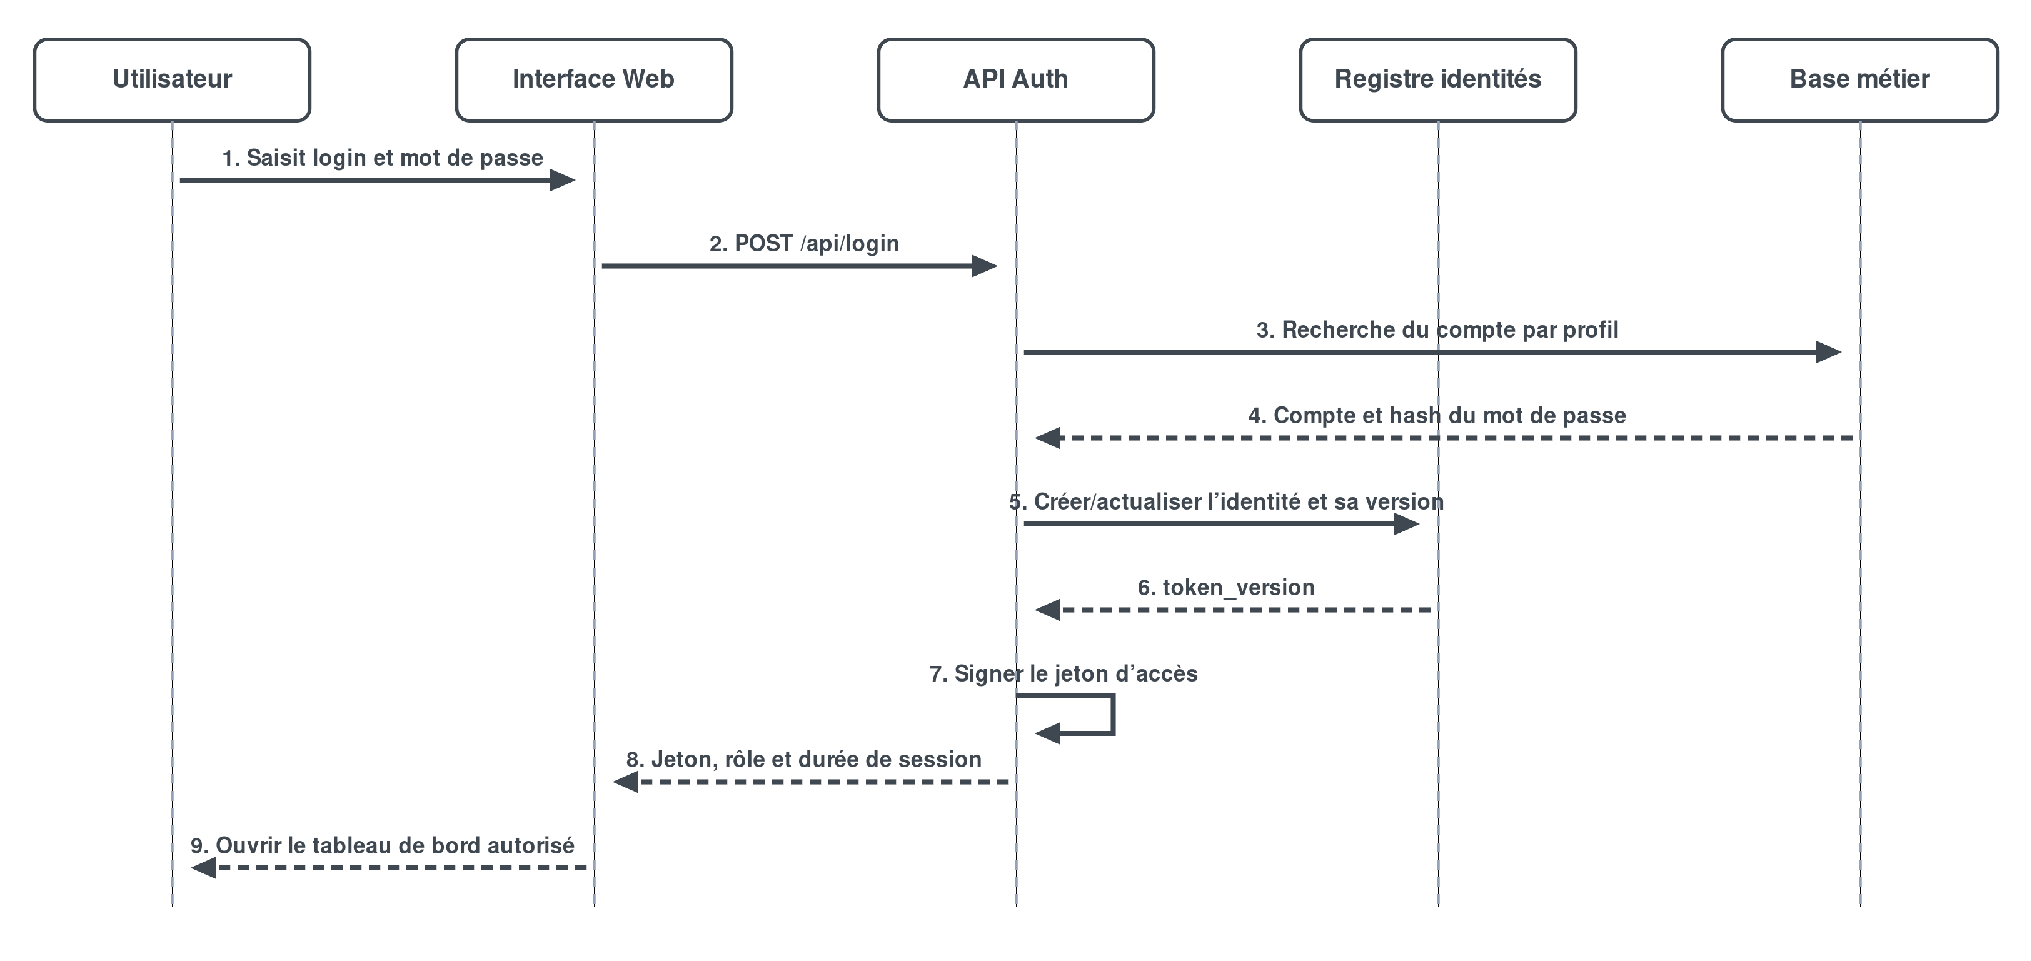
\includegraphics{figures/argos_05_sequence_authentification.pdf}%
}
\caption{Séquence d'authentification signée}
\label{fig-argos-seq-auth}
\tablesourcepromoteurs

\end{figure}

La sécurisation des accès et l'initialisation du parc logistique reposent sur des chaînes de transactions univoques qui garantissent l'intégrité de la plateforme. La séquence d'authentification formalise le processus d'accès par jetons signés : lors de la tentative de connexion d'un utilisateur, le système valide les informations d'identification au sein de la table de profils dédiée, synchronise le registre central des identités et génère un jeton sécurisé dont la validité est contrôlée à chaque requête par l'intermédiaire de la version de la clé (\texttt{token\_version}) et de l'état du compte.

\begin{figure}[htbp]
\centering
\resizebox{0.85\textwidth}{!}{%
  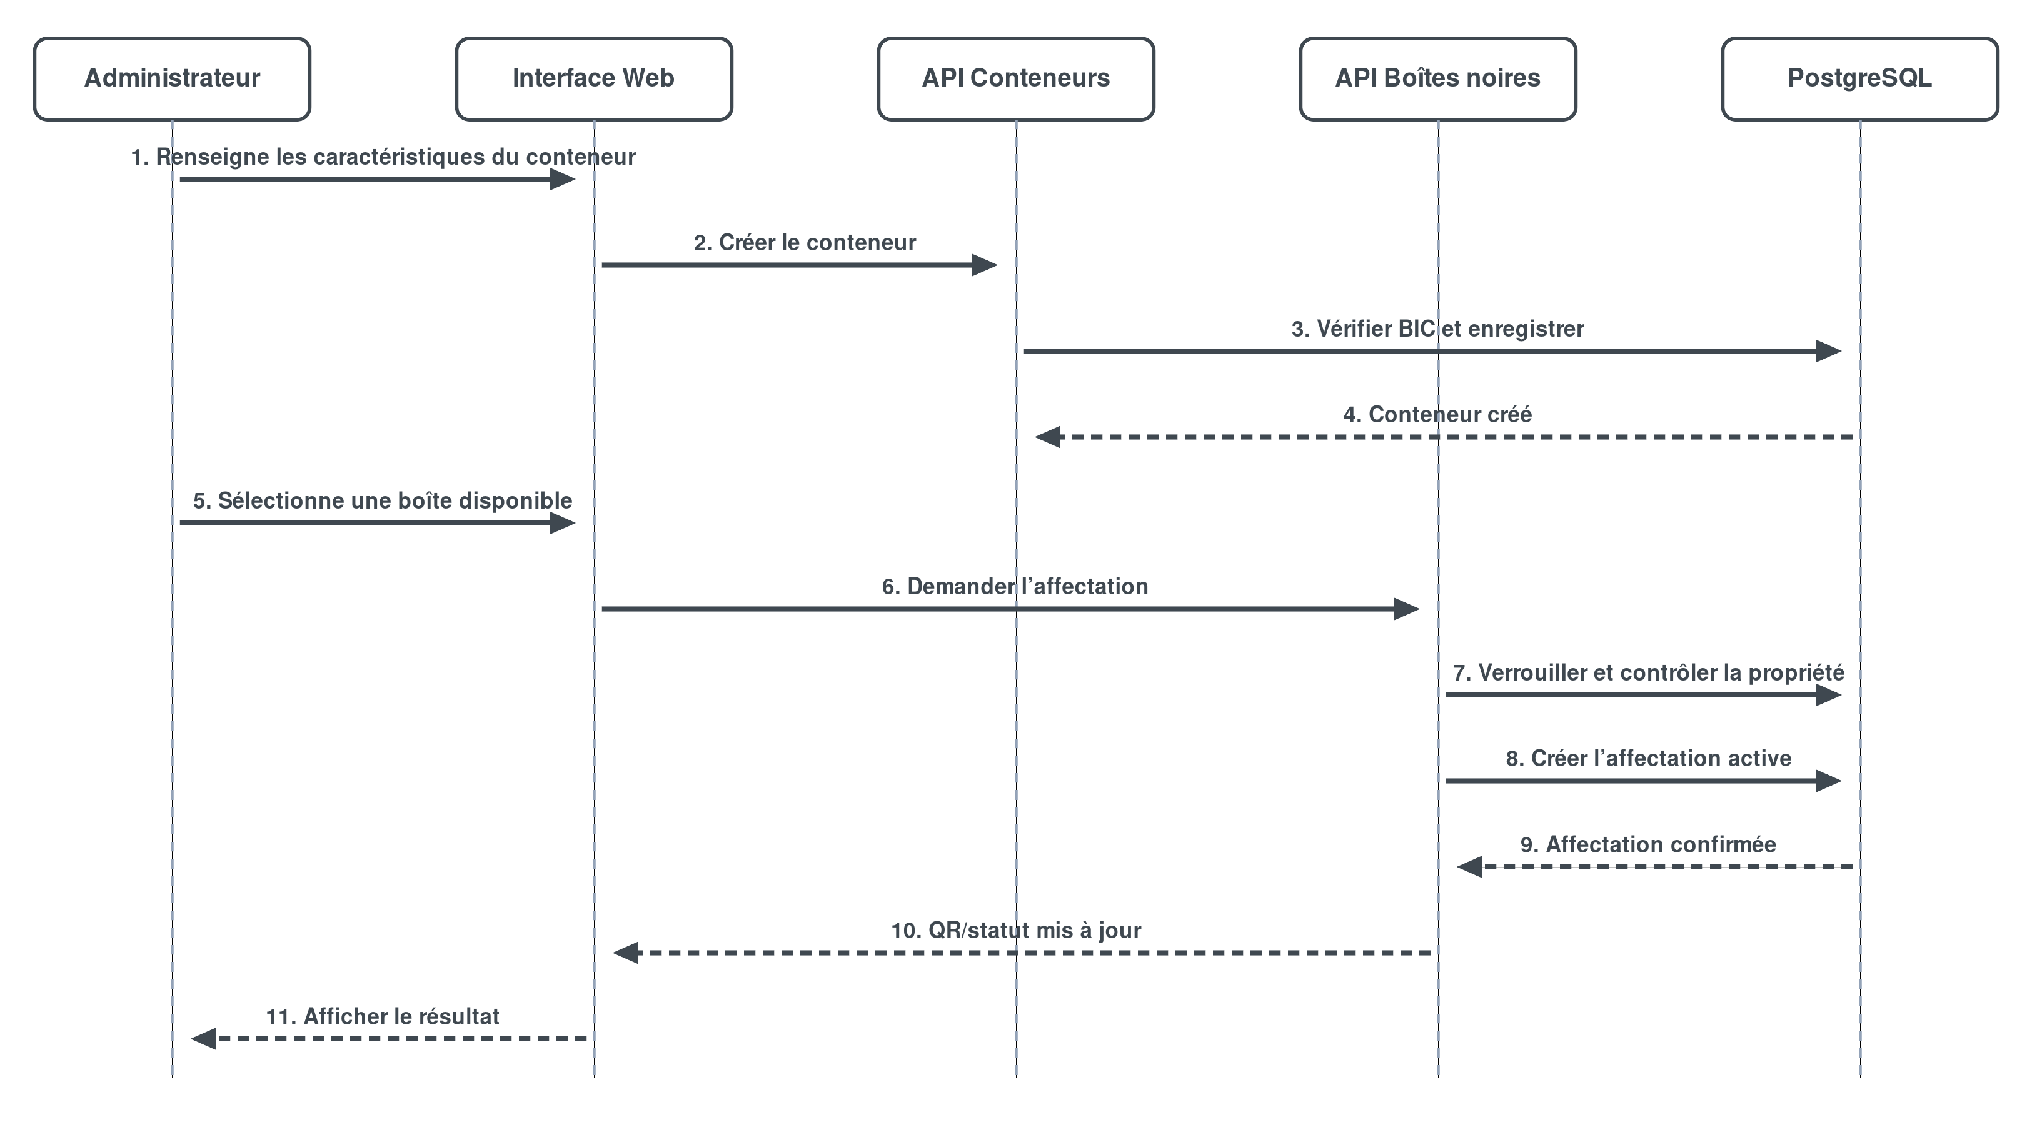
\includegraphics{figures/argos_06_sequence_gestion_conteneur_boite.pdf}%
}
\caption{Séquence de création et d'affectation conteneur--boîte}
\label{fig-argos-seq-affectation}
\tablesourcepromoteurs

\end{figure}

Le diagramme de gestion et d'affectation orchestre la création des unités logistiques. Le système réceptionne l'identifiant du conteneur, l'enrichit et le normalise dynamiquement via l'interopérabilité avec les services d'API externes (notamment l'API BIC), avant d'effectuer l'association transactionnelle avec un boîtier disponible dans le parc. Ce couplage garantit qu'aucune entité physique n'évolue sans rattachement traçable.


\subsubsection{Contrat et enrôlement IoT}

\begin{figure}[htbp]
\centering
\resizebox{0.85\textwidth}{!}{%
  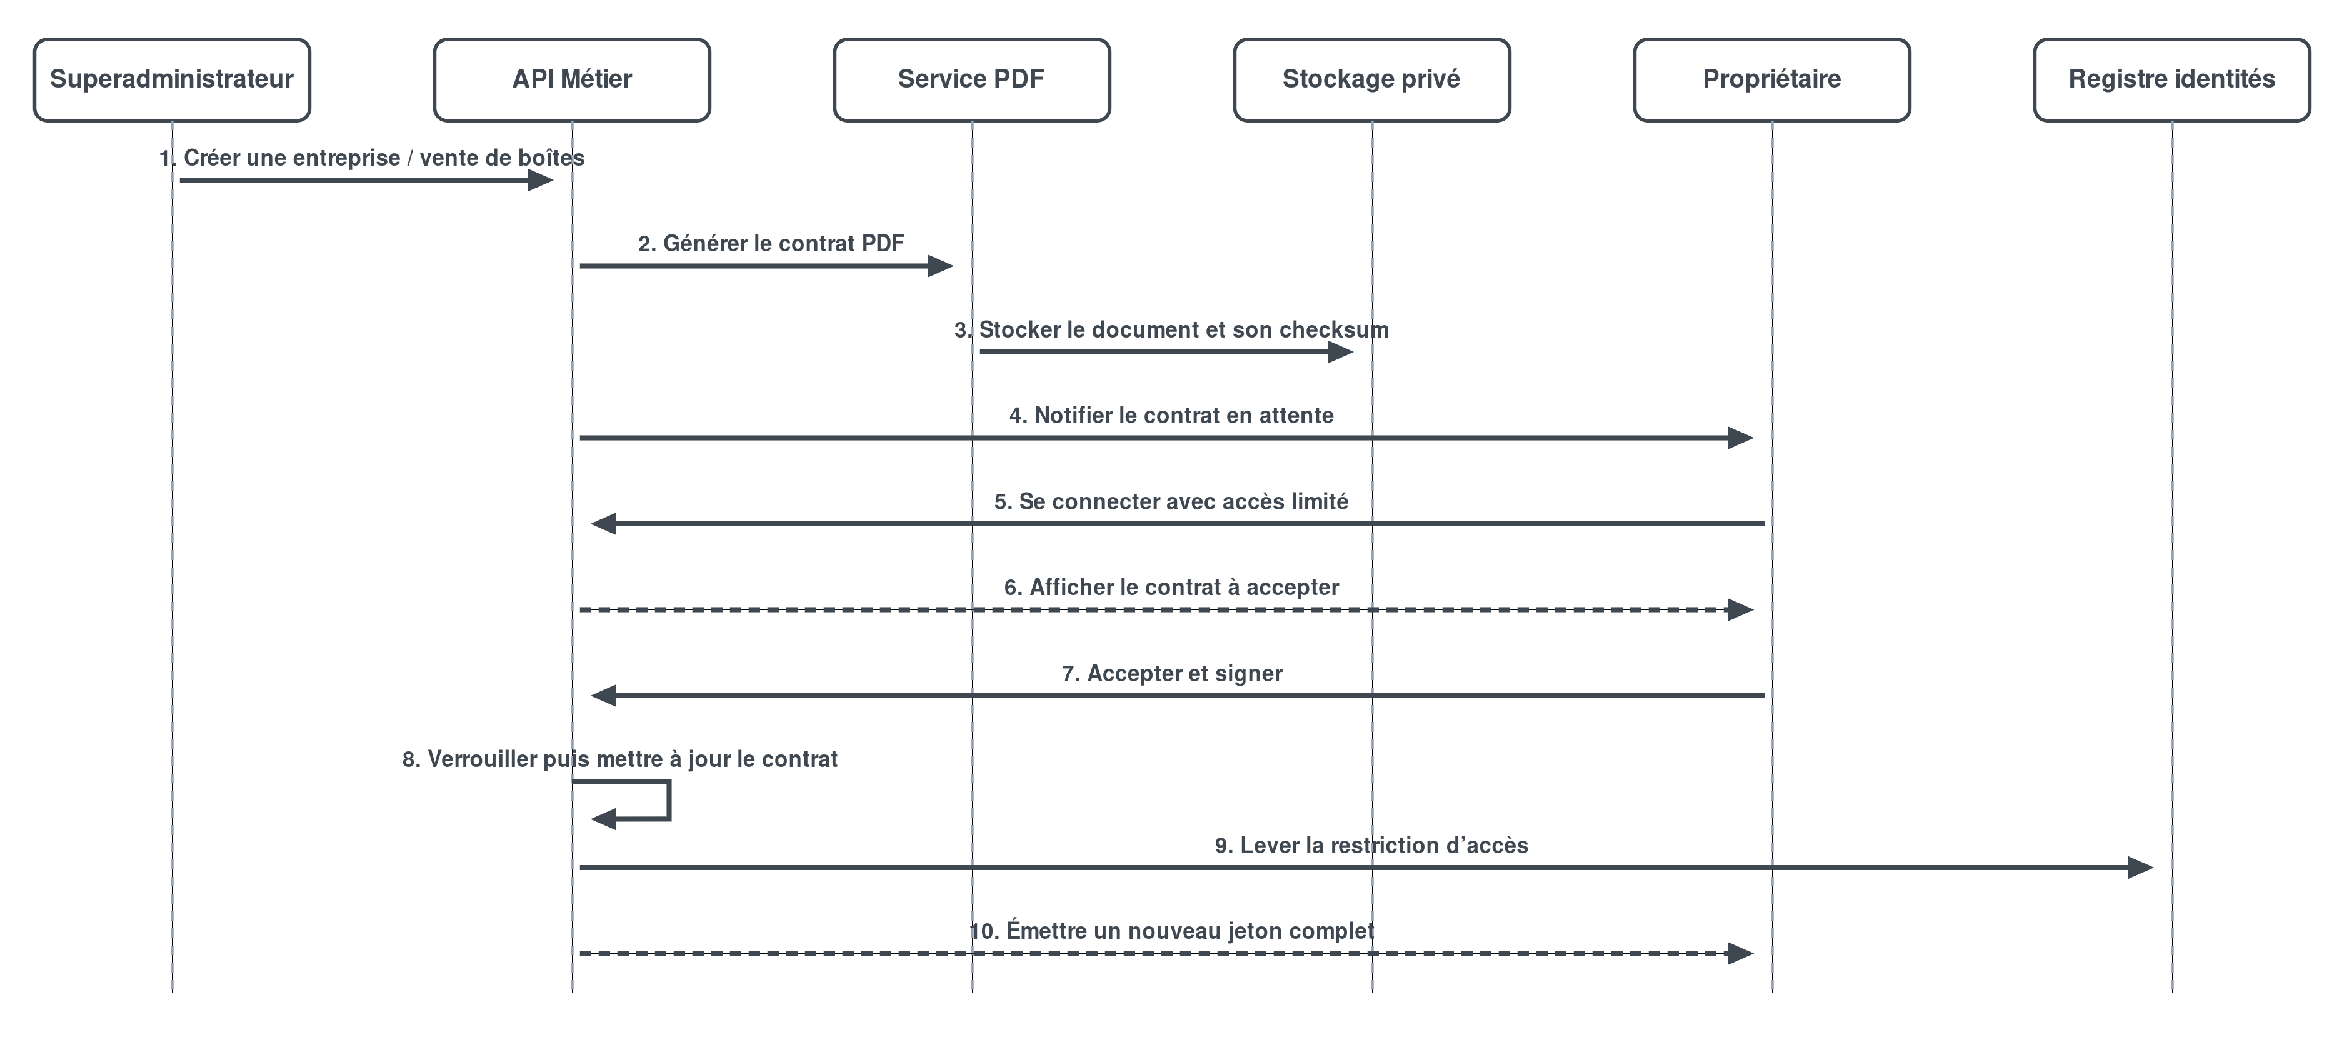
\includegraphics{figures/argos_07_sequence_contrat.pdf}%
}
\caption{Séquence de génération et d'acceptation d'un contrat}
\label{fig-argos-seq-contrat}
\tablesourcepromoteurs

\end{figure}

Le cycle de contractualisation et de provisionnement matériel matérialise la transition entre la gestion administrative et l'exploitation technique sur le terrain. Le diagramme de séquence des contrats retrace la chaîne décisionnelle allant de l'initiation de l'entreprise par le superadministrateur jusqu'à la signature numérique et l'archivage sécurisé du document dans le stockage privé. Cette validation lève automatiquement les restrictions d'accès initiales dans le registre d'identités et octroie au propriétaire ses pleines prérogatives opérationnelles.

\begin{figure}[htbp]
\centering
\resizebox{0.85\textwidth}{!}{%
  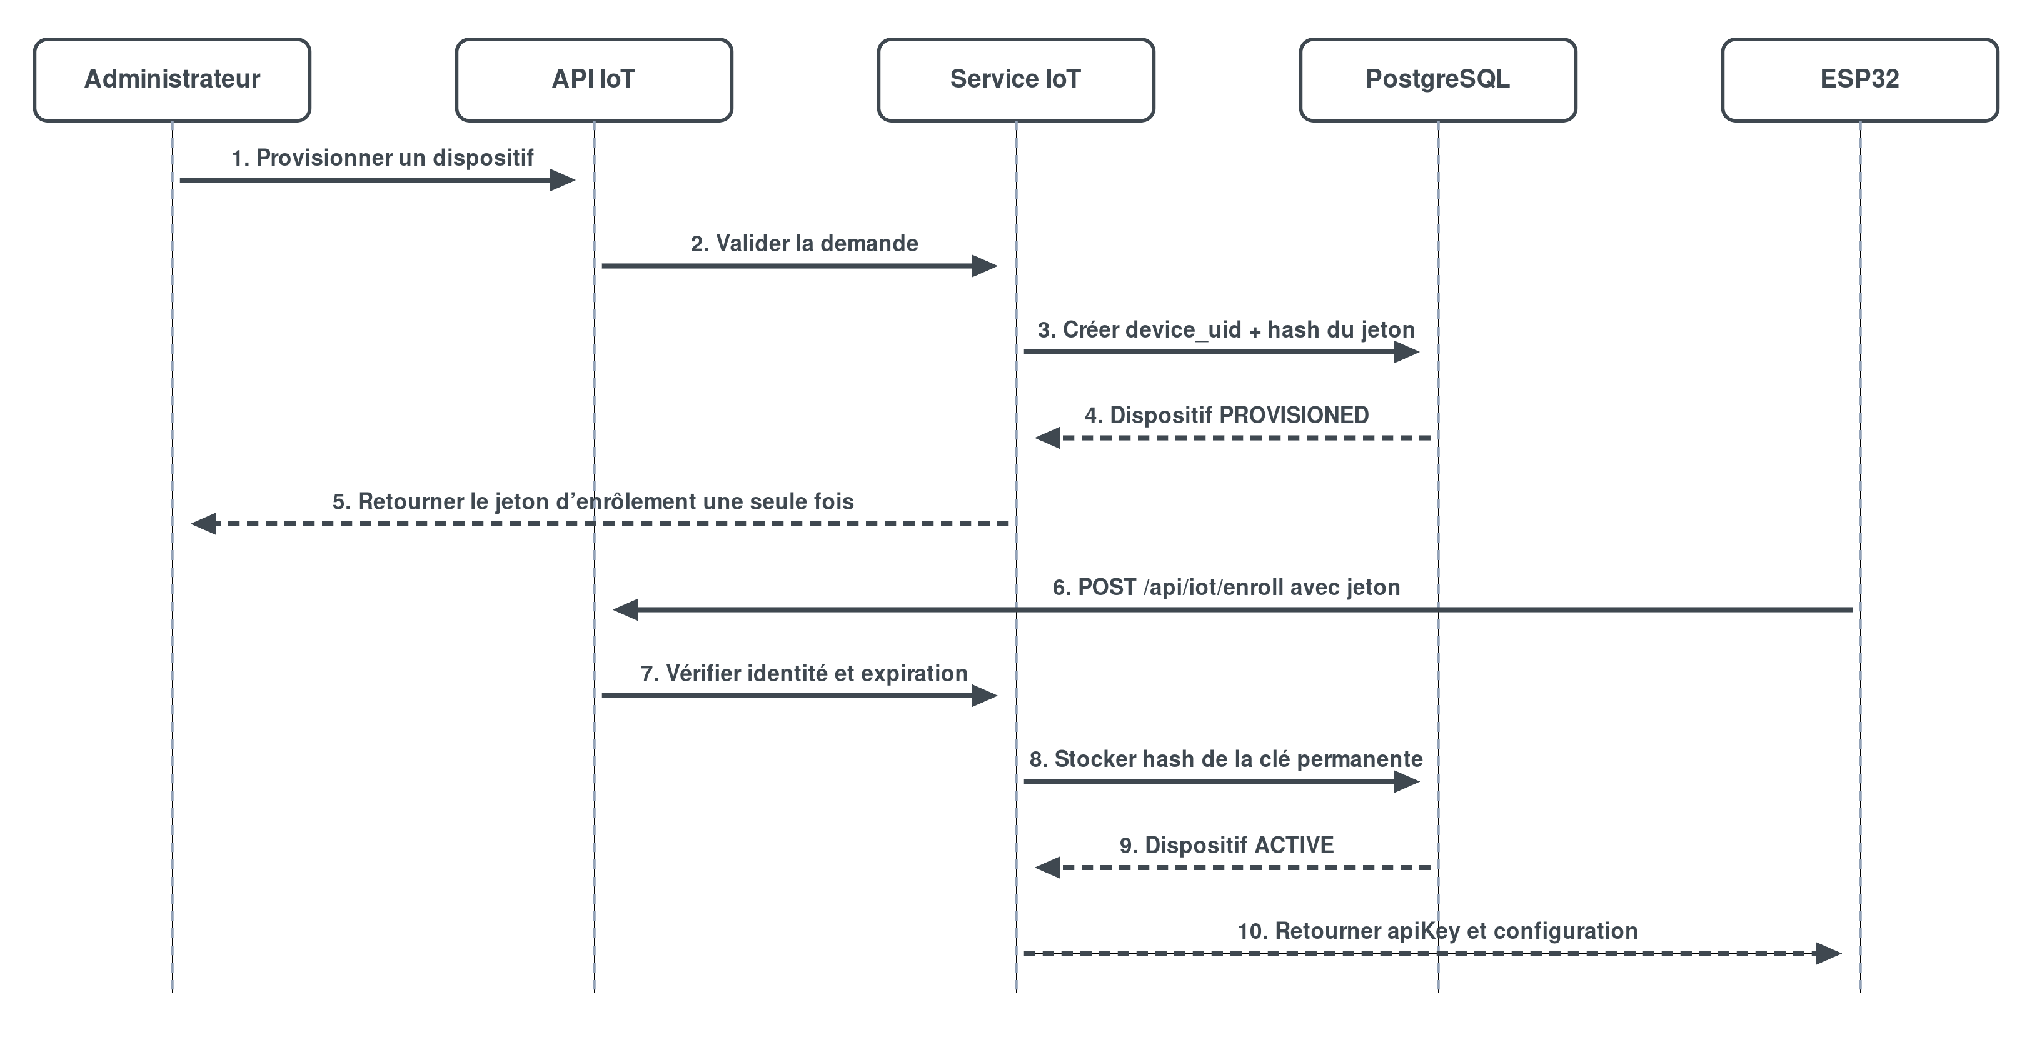
\includegraphics{figures/argos_08_sequence_enrolement_iot.pdf}%
}
\caption{Séquence de provisionnement et d'enrôlement d'un ESP32}
\label{fig-argos-seq-enrolement}
\tablesourcepromoteurs

\end{figure}

Dans la continuité, le processus d'enrôlement de l'ESP32 formalise le mécanisme d'initialisation sécurisée du dispositif embarqué. À partir d'un jeton temporaire valable par défaut 24 heures, le système authentifie le matériel, génère une empreinte, supprime le jeton initial après validation et délivre une clé permanente, faisant basculer l'état du boîtier à l'état \code{ACTIVE} au sein de la flotte.


\subsubsection{Télémétrie, commande, voyage et déstockage}

\begin{figure}[htbp]
\centering
\resizebox{0.85\textwidth}{!}{%
  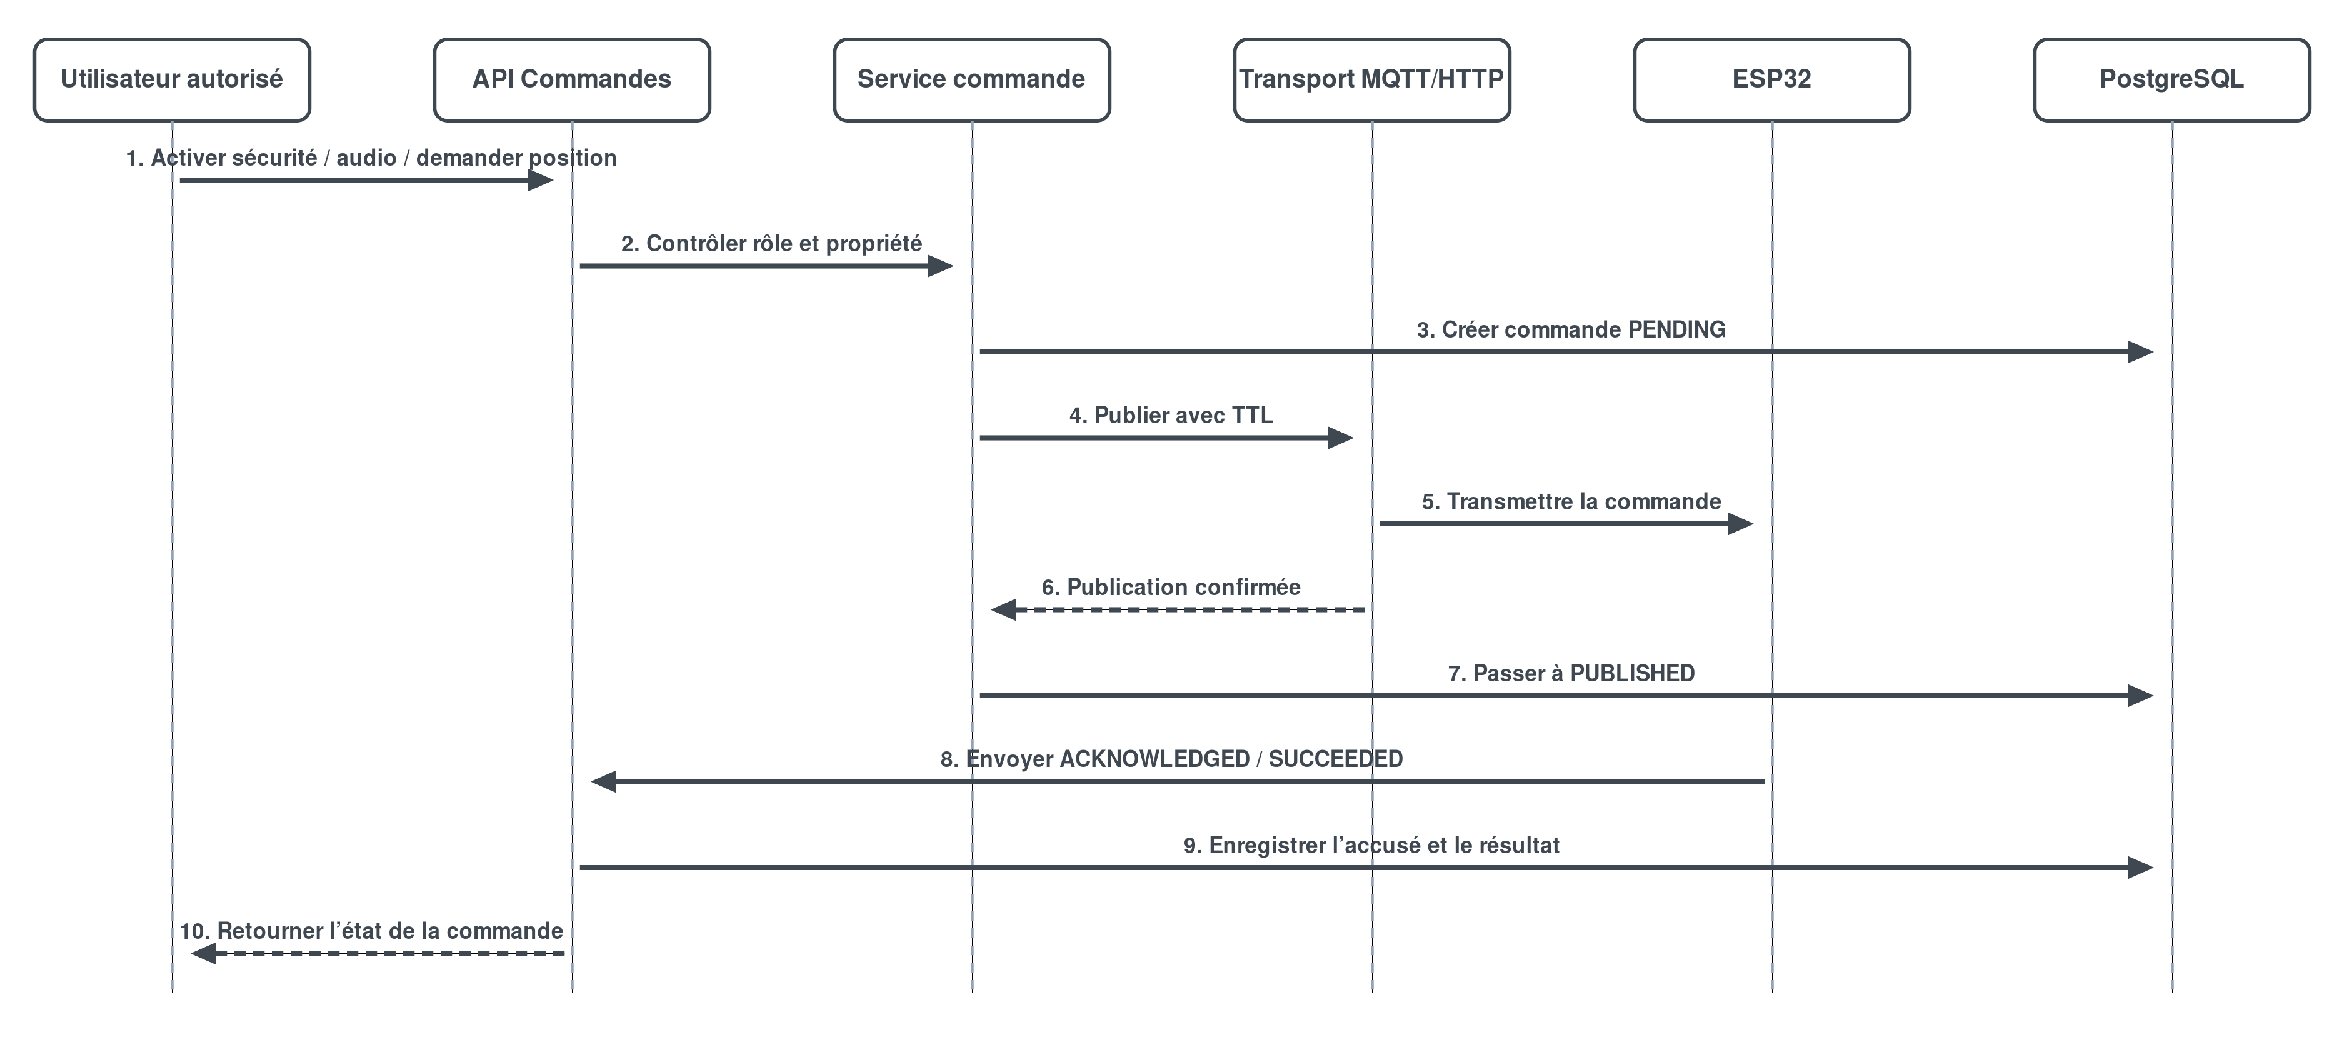
\includegraphics{figures/argos_10_sequence_commande_iot.pdf}%
}
\caption{Séquence d'émission et d'acquittement d'une commande}
\label{fig-argos-seq-commande}
\tablesourcepromoteurs

\end{figure}

L'exploitation quotidienne de la solution s'appuie sur des flux dynamiques complexes. Concernant le pilotage matériel, le diagramme d'émission de commandes illustre la boucle de transmission à distance vers les boîtiers. Les commandes transitent par des états stricts (\code{PENDING}, \code{PUBLISHED}, \code{ACKNOWLEDGED}, \code{SUCCEEDED}, \code{FAILED} ou \code{EXPIRED}), l'acquittement portant explicitement sur le \code{deviceUid} pour certifier l'exécutant.

\begin{figure}[htbp]
\centering
\resizebox{0.85\textwidth}{!}{%
  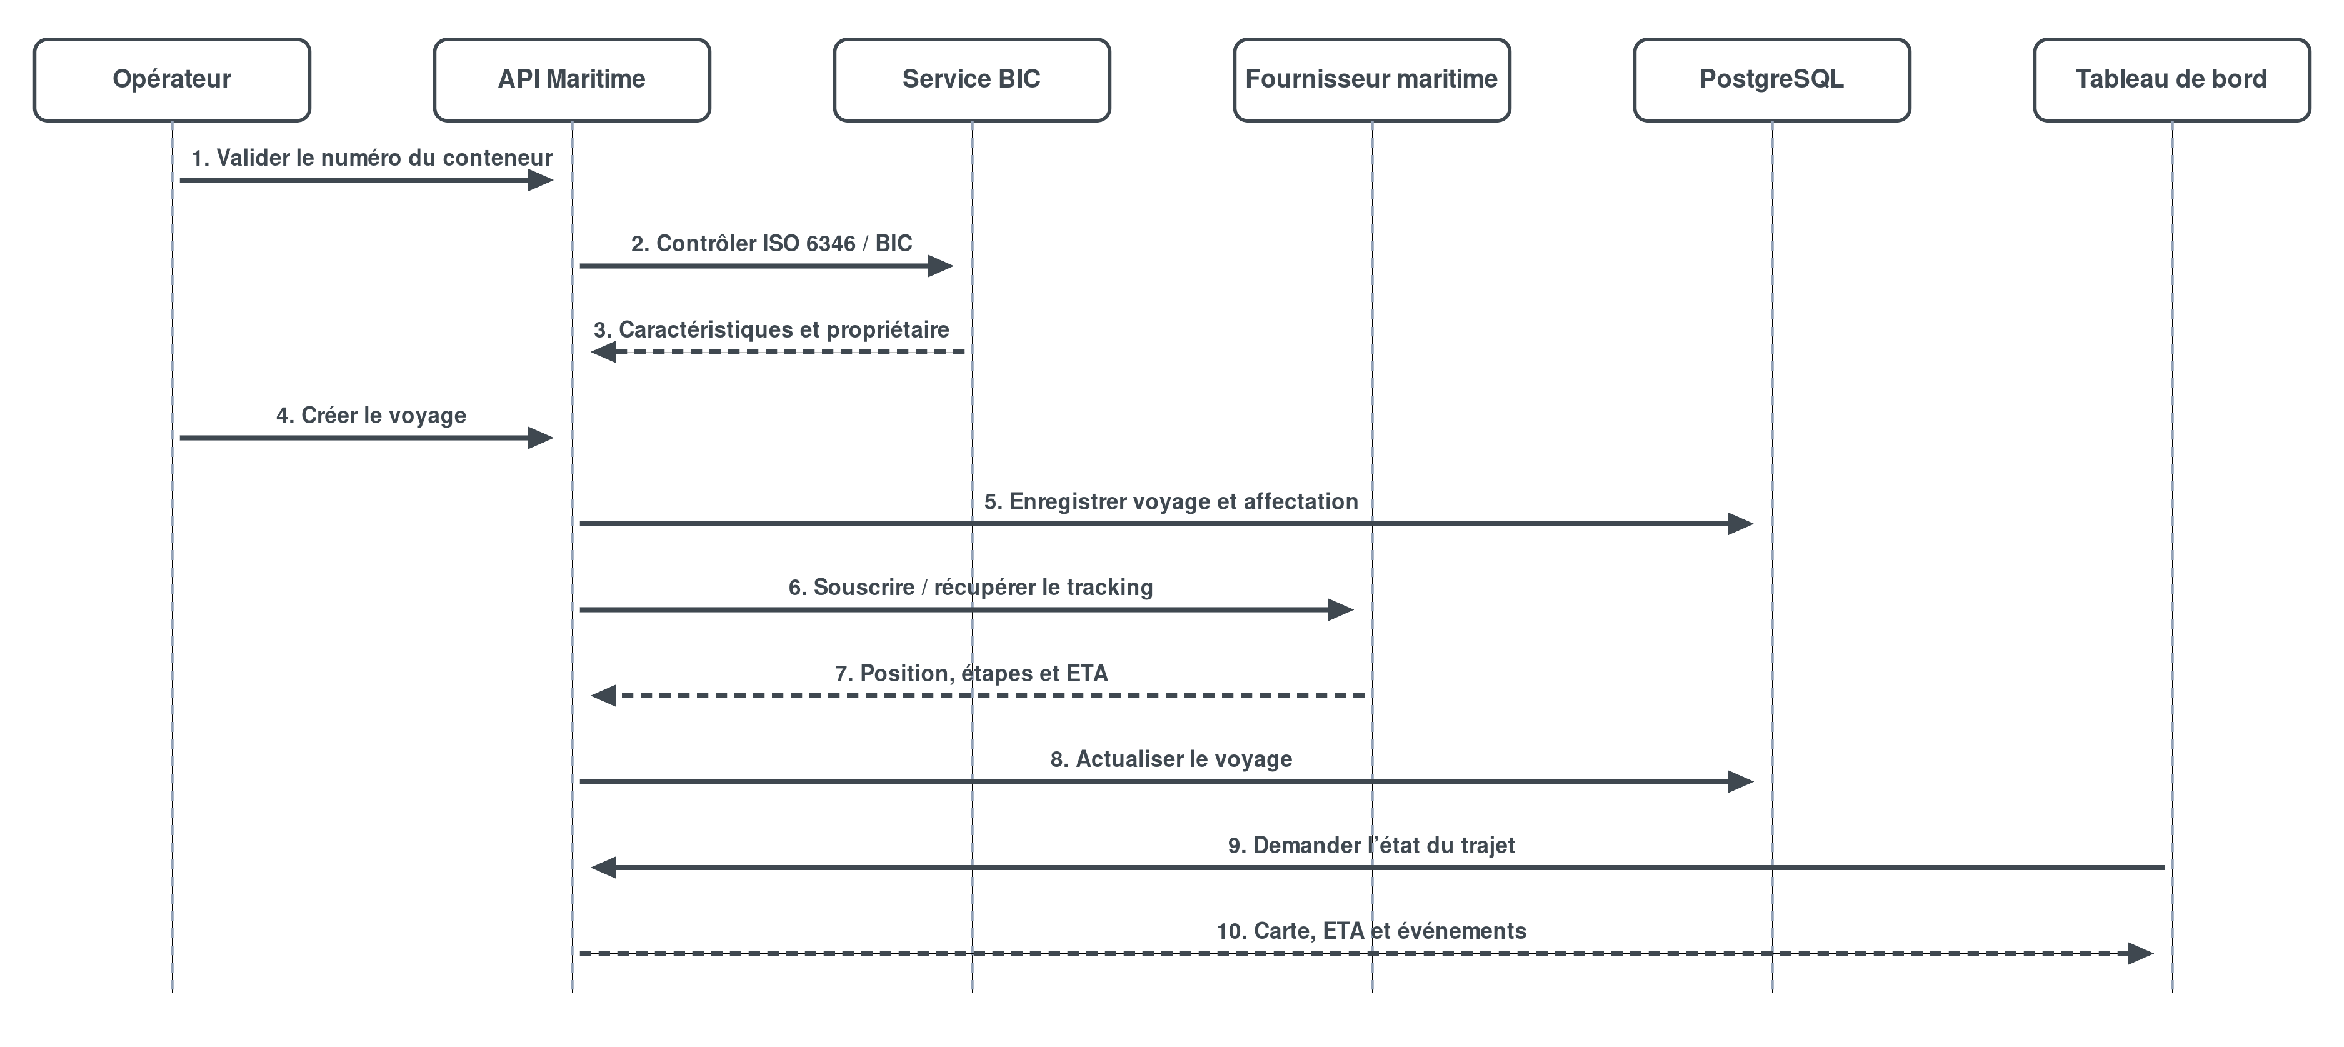
\includegraphics{figures/argos_11_sequence_voyage_tracking.pdf}%
}
\caption{Séquence de création et de suivi d'un voyage maritime}
\label{fig-argos-seq-voyage}
\tablesourcepromoteurs

\end{figure}

Le suivi des voyages maritimes met en évidence le rapprochement analytique entre la position GPS autonome du conteneur (transmise par la télémétrie IoT) et les données AIS du navire porteur. Cette corrélation permet d'anticiper les litiges, d'identifier le port le plus proche et de calculer précisément les distances de transport.

\begin{figure}[htbp]
\centering
\resizebox{0.85\textwidth}{!}{%
  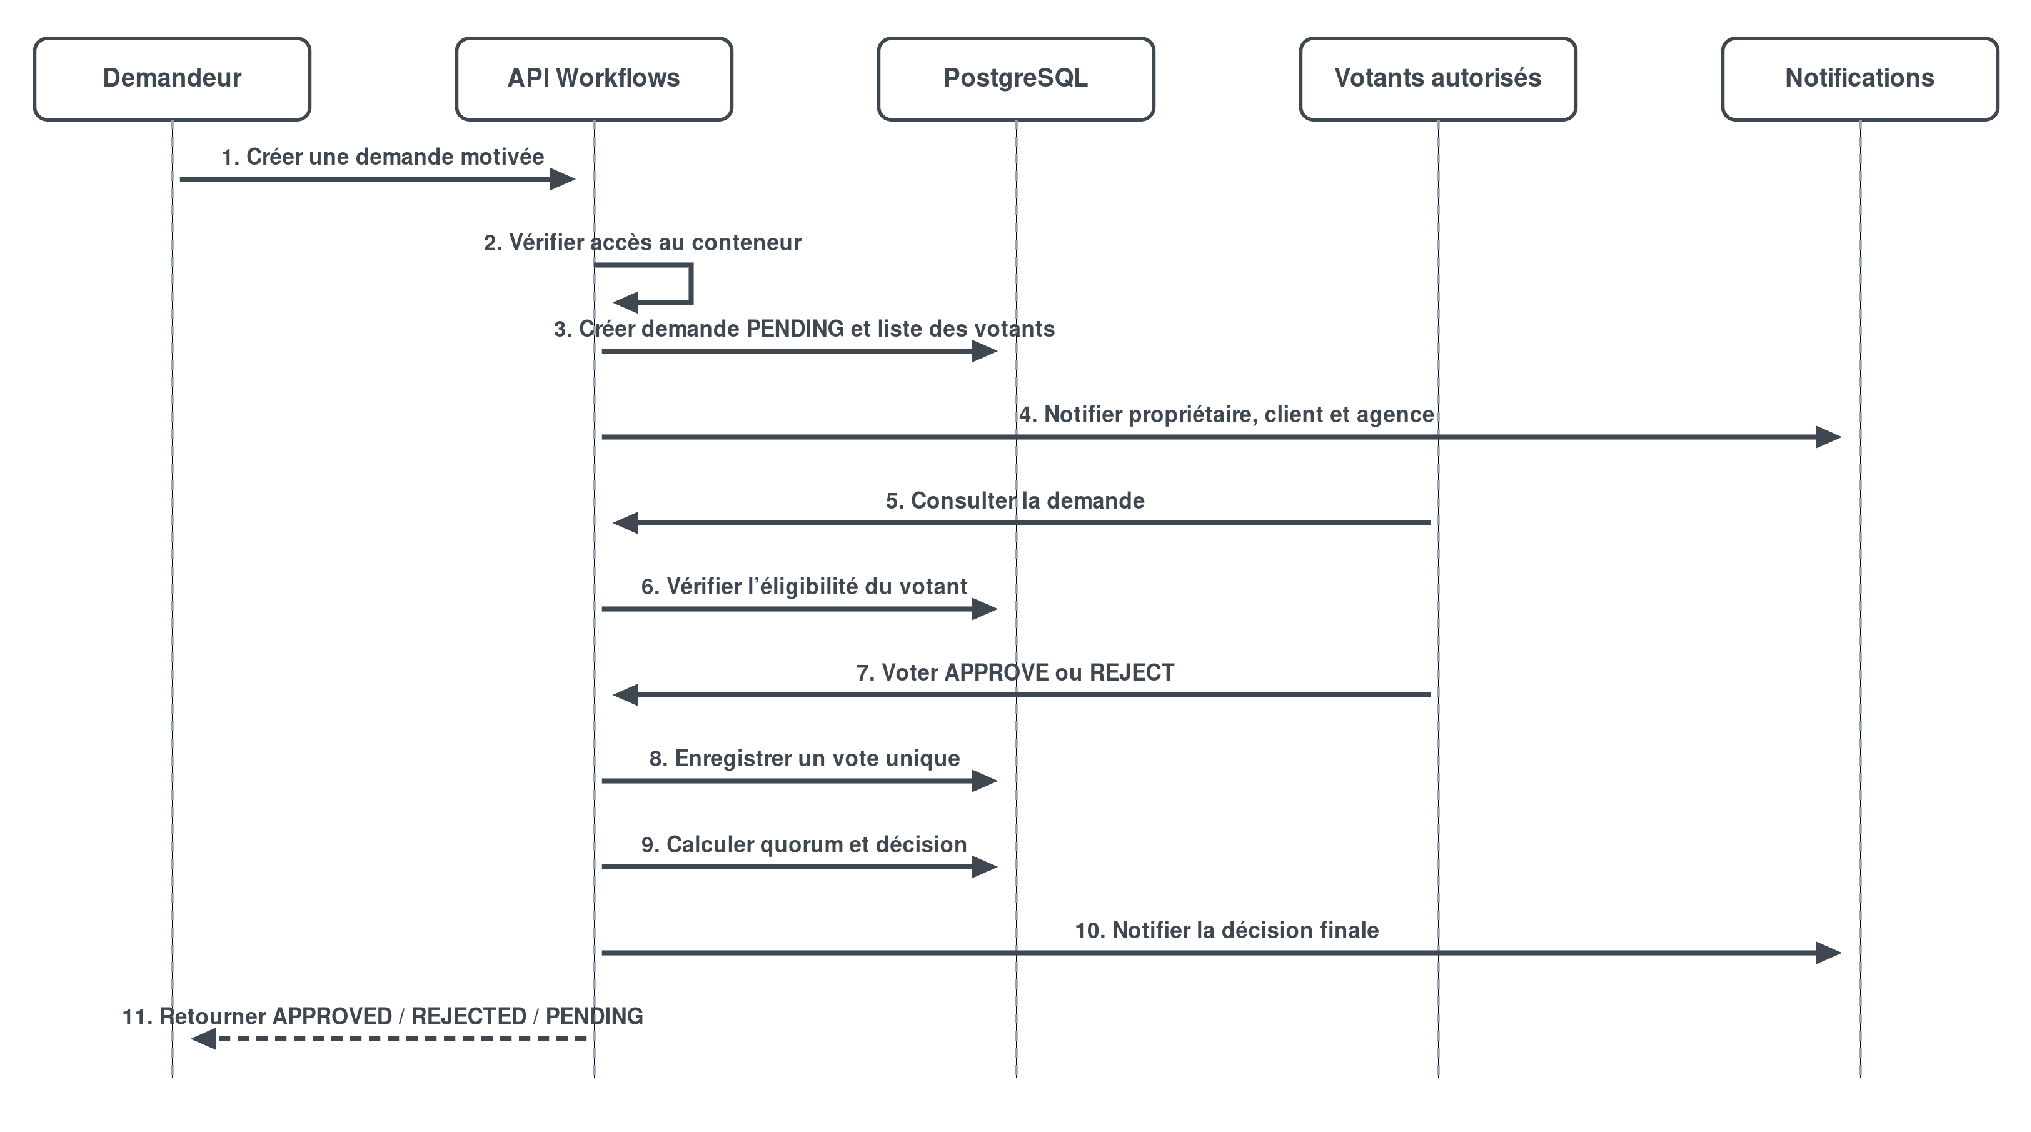
\includegraphics{figures/argos_12_sequence_destockage.pdf}%
}
\caption{Séquence de demande, vote et décision de déstockage}
\label{fig-argos-seq-destockage}
\tablesourcepromoteurs

\end{figure}

Enfin, le processus de déstockage formalise un workflow décisionnel collaboratif et sécurisé : l'émission d'une demande identifiant les votants et l'échéance déclenche une procédure d'approbation multipartite. À l'issue des votes requis, le worker automatisé génère le rapport final d'expertise, détache la boîte du conteneur et maintient temporairement l'accès selon le paramètre \code{visibility\_until}.

% \\\\\\\\\\\\\\\\\\\\\\\\\\\\\\\\\\\
\subsubsection{Chaîne de télémétrie de bout en bout}

\begin{figure}[htbp]
\centering
\resizebox{0.95\textwidth}{!}{%
  \resizebox{!}{0.82\textheight}{%
\begin{tikzpicture}[
  font=\sffamily\small,
  lane/.style={draw=argosrule,rounded corners=3pt,fill=argospale,
    minimum width=4.2cm,minimum height=1.15cm,align=center},
  procstep/.style={draw=argosmid,rounded corners=3pt,fill=white,
    minimum width=4.6cm,minimum height=1.15cm,align=center,line width=.8pt},
  store/.style={draw=argosnavy,cylinder,shape border rotate=90,aspect=.24,
    fill=argoslight,minimum width=4.3cm,minimum height=1.45cm,align=center,line width=.9pt},
  decision/.style={draw=argosnavy,diamond,aspect=2.25,fill=argospale,
    minimum width=4.5cm,minimum height=1.5cm,align=center,line width=.9pt},
  flow/.style={draw=argosgray,line width=.85pt,-{Stealth[length=2.4mm]}},
  async/.style={draw=argosmid,dashed,line width=.85pt,-{Stealth[length=2.4mm]}},
  note/.style={font=\sffamily\scriptsize,align=center,text=argosgray}
]
\node[lane] (sta) at (-9.6,7.4) {ESP32 en mode station\\POST \texttt{/api/iot/telemetry}\\clé \texttt{X-Device-Key}};
\node[lane] (ap) at (0,7.4) {ESP32 en point d'accès\\GET local \texttt{/api/v1/telemetry}\\toutes les 1 à 30 s (2 s par défaut)};
\node[lane] (browser) at (9.6,7.4) {Navigateur ARGOS authentifié\\vérification de l'UID, affichage immédiat\\et file FIFO locale bornée};
\node[procstep] (route) at (0,5.1) {Route commune d'ingestion\\standard ou \texttt{direct-telemetry}};
\node[procstep] (validate) at (0,3.1) {Valider UUID, \texttt{deviceUid}, boîte,\\conteneur, horodatage, séquence et plages};
\node[decision] (identity) at (0,.8) {Identité, affectation\\et séquence valides ?};
\node[store] (rawreject) at (-8.0,-1.7) {PostgreSQL (voie standard)\\message brut rejeté\\et motif};
\node[procstep] (normalise) at (0,-1.7) {Normaliser la qualité capteur\\et remplacer GPS 0,0 par un\\repli navigateur déjà autorisé};
\node[procstep] (threshold) at (-7.6,-4.4) {Comparer aux seuils\\et construire les alertes};
\node[store] (redis) at (0,-4.4) {Redis\\clé latest (TTL 24 h)\\+ stream borné à 10 000};
\node[store] (postgres) at (7.6,-4.4) {PostgreSQL\\raw, lectures, positions, événements,\\notifications et audit (transaction)};
\node[procstep] (liveapi) at (-5.1,-7.1) {\texttt{/api/stats/live}\\Redis d'abord, PostgreSQL en repli};
\node[procstep] (ui) at (0,-9.1) {Partager la mesure dans l'application\\carte, boîtes, statistiques, alertes, événements};
\node[procstep] (notify) at (7.0,-7.1) {Notifier les parties liées\\application et courriel, avec anti-doublon};

\draw[flow] (sta.south) -- (route.north west);
\draw[flow] (ap.east) -- (browser.west);
\draw[flow] (browser.south) |- node[note,pos=.25,right]{POST Bearer} (route.east);
\draw[flow] (route) -- (validate);
\draw[flow] (validate) -- (identity);
\draw[flow] (identity.west) -- node[note,above]{non} (rawreject.east);
\draw[flow] (identity) -- node[note,right]{oui} (normalise);
\draw[flow] (normalise.west) to[out=200,in=70] (threshold.north);
\draw[flow] (threshold.east) -- (redis.west);
\draw[flow] (redis.east) -- (postgres.west);
\draw[flow] (redis) -- (liveapi);
\draw[flow] (liveapi) -- (ui.north west);
\draw[flow] (browser.south east) |- node[note,pos=.24,right]{rendu local avant synchronisation} (ui.east);
\draw[async] (postgres) -- (notify);
\draw[async] (notify.south) |- (ui.east);
\end{tikzpicture}%
}
%
}
\caption{Chaîne de télémétrie de bout en bout}
\label{fig-argos-flux-telemetrie}
\tablesourcepromoteurs

\end{figure}

\subsubsection{Fichiers JSON de télémétrie}

\begingroup
\small
\begin{longtable}{@{}p{4.7cm}p{2.5cm}p{6.8cm}@{}}
\caption{Champs du message de télémétrie et règles de validation}
\label{tab-contrat-telemetrie}\\
\tableheadrow \thc{Chemin JSON} & \thc{Type} & \thc{Règle et utilisation} \\
\midrule
\endfirsthead
\tableheadrow \thc{Chemin JSON} & \thc{Type} & \thc{Règle et utilisation} \\
\midrule
\endhead
\code{messageId} & UUID & Identifiant de message unique ; doublon traité de manière idempotente \\
\hline
\code{type} & chaîne & Valeur obligatoire \code{telemetry} \\
\hline
\code{deviceUid} & chaîne & Identité unique du matériel, comparée à \code{iot\_devices.device\_uid} \\
\hline
\code{blackBoxId} & entier positif & Doit correspondre à l'association active du dispositif \\
\hline
\code{containerId} & chaîne ou nul & Normalisé en majuscules et contrôlé si une affectation existe \\
\hline
\code{timestamp} & ISO-8601 & Fuseau accepté ; écart maximal de six heures avec le serveur \\
\hline
\code{sequence} & entier $\geq 0$ & Doit être strictement supérieur à la dernière séquence traitée \\
\hline
\code{position.latitude} & réel & Intervalle $[-90,90]$ \\
\hline
\code{position.longitude} & réel & Intervalle $[-180,180]$ \\
\hline
\code{position.accuracy} & réel & Intervalle $[0,100000]$ mètres \\
\hline
\code{position.speed} & réel & Intervalle $[0,1000]$ ; affiché et comparé au seuil \\
\hline
\code{position.heading} & réel & Intervalle $[0,360]$ degrés \\
\hline
\code{position.source} & chaîne & \code{ESP32}, \code{DIRECT\_WIFI} ou \code{BROWSER\_FALLBACK} \\
\hline
\code{sensors.temperature} & réel & $[-80,120]$ \textdegree C ; neutralisé si DHT invalide \\
\hline
\code{sensors.humidity} & réel & $[0,100]$ \% ; neutralisé si DHT invalide \\
\hline
\code{sensors.shock} & réel & $[0,200]$ g ; neutralisé si MPU invalide \\
\hline
\code{sensors.pressure} & réel & $[300,1200]$ hPa ; neutralisé si non mesuré \\
\hline
\code{sensors.flameDetected} & booléen & Déclenche une alerte si vrai \\
\hline
\code{sensors.doorOpen} & booléen & Déclenche une alerte lorsque la sécurité est active \\
\hline
\code{sensors.batteryLevel} & réel & $[0,100]$ \% ; neutralisé si valeur non mesurée \\
\hline
\code{sensors.lightLevel} & réel & Valeur optionnelle $[0,4095]$ \\
\hline
\code{sensors.soundLevel} & réel & Valeur optionnelle $[0,4095]$ \\
\hline
\code{sensors.distanceCm} & réel & Valeur optionnelle $[0,1000]$ cm \\
\hline
\nolinkurl{sensors.accelerationX/Y/Z} & réels & Valeurs optionnelles dans $[-200,200]$ \\
\hline
\code{sensors.securityAlarm} & booléen & État synthétique de l'alarme locale \\
\hline
\code{modes.securityEnabled} & booléen & Sécurité des portes activée ou bloquée \\
\hline
\nolinkurl{modes.audioRecordingEnabled} & booléen & État de l'enregistrement audio \\
\hline
\nolinkurl{modes.audioListeningEnabled} & booléen & État de l'écoute audio \\
\hline
\nolinkurl{modes.flameDetectionEnabled} & booléen & État de la détection de flamme \\
\hline
\code{quality.dhtValid} & booléen & Fiabilité température/humidité \\
\hline
\code{quality.mpuValid} & booléen & Fiabilité choc/accélérations \\
\hline
\code{quality.gpsValid} & booléen & Validité du GPS embarqué \\
\hline
\code{quality.distanceValid} & booléen & Validité de la distance ultrasonique \\
\hline
\code{quality.sdReady} & booléen & Disponibilité de la carte SD \\
\hline
\code{quality.pressureMeasured} & booléen & Distingue une mesure réelle d'une valeur de substitution \\
\hline
\code{quality.batteryMeasured} & booléen & Distingue une mesure réelle d'une estimation \\
\hline
\code{quality.timestampSource} & chaîne & Origine de l'heure, appareil ou navigateur/API \\
\tablebottomrule
\end{longtable}
\tablesourcepromoteurs
\endgroup

\subsubsection{Ordre de traitement}

Après validation et contrôle de l'association, l'application applique le
repli de position et transforme en \code{NULL} les capteurs déclarés
invalides. Elle publie ensuite le document normalisé dans Redis DB1. La même
requête insère les vues durables dans PostgreSQL et valide la transaction.
L'ordre logique est donc :
\[
\text{route de télémétrie}
\rightarrow \text{validation}
\rightarrow \text{Redis temps réel}
\rightarrow \text{PostgreSQL durable}.
\]

Le message brut est préparé dans la transaction PostgreSQL pour conserver le
JSON reçu. La voie distante tente également de journaliser les messages
rejetés ; la voie directe annule actuellement sa transaction en cas de rejet.

\subsubsection{Propagation de l'identité et de la séquence}

\begin{table}[htbp]
\centering
\caption{Traçabilité de l'UID et de la séquence dans chaque représentation}
\label{tab-tracabilite-uid-sequence}
\begin{tabularx}{\textwidth}{@{}p{3.6cm}p{5.0cm}X@{}}
\tableheadrow \thc{Destination} & \thc{Identité} & \thc{Séquence et lien} \\
\midrule
Redis latest/stream & \code{deviceUid} direct & \code{sequence} directe et \code{messageId} \\
\hline
\code{iot\_raw\_messages} & \code{device\_uid} direct & \code{message\_id} pointe vers le JSON contenant la séquence \\
\hline
\code{sensor\_readings} & \code{device\_id} vers \code{iot\_devices} & \code{sequence} directe et \code{raw\_message\_id} \\
\hline
\code{positions} & \code{device\_id} vers \code{iot\_devices} & Lien \code{raw\_message\_id} vers le message et sa séquence \\
\hline
\code{evenement\_save} & \code{device\_uid} direct & \code{sequence} directe, boîte et horodatage \\
\hline
\code{notifications} & \code{device\_uid} direct pour les alertes IoT & \code{sequence} directe et boîte concernée \\
\hline
\code{audit\_logs} & UID dans \code{entity\_id} & Séquence et UUID dans \code{details} JSONB \\
\tablebottomrule
\end{tabularx}
\tablesourcepromoteurs
\end{table}

Cette propagation permet de trier les mesures par dispositif, détecter un
trou ou un rejeu de séquence, et relier une alerte à la mesure qui l'a
produite, même lorsque la table concernée ne duplique pas physiquement les
deux colonnes.

\subsubsection{Partage distant et QR code}

À l'ouverture d'une session directe unique, ARGOS crée une notification avec
le lien distant et évite une nouvelle annonce pendant 30 minutes pour le
même acteur. Si la boîte est liée à un conteneur, le propriétaire, les agences
actives et les clients abonnés ayant une adresse valide reçoivent le lien et
le QR code par courriel. Le scan n'annule pas les restrictions : une
authentification ARGOS et un lien actif avec la ressource restent obligatoires.
Pour une boîte non affectée, l'information demeure dans le périmètre du
superadministrateur.

\subsubsection{Sécurité des portes et diffusion des alertes}

\begin{figure}[htbp]
\centering
\resizebox{0.95\textwidth}{!}{%
  % Activation/désactivation du mode sécurité, avec variantes directe et distante.
\resizebox{\textwidth}{!}{%
\begin{tikzpicture}[
  font=\sffamily\small,
  participant/.style={draw=argosnavy,rounded corners=2pt,fill=argoslight,
    minimum width=3.6cm,minimum height=1.1cm,align=center,line width=.9pt,font=\sffamily\small\bfseries},
  life/.style={draw=argosrule,dashed,line width=.8pt},
  call/.style={draw=argosgray,line width=.9pt,-{Stealth[length=2.5mm]}},
  reply/.style={draw=argosgray,dashed,line width=.85pt,-{Stealth[length=2.5mm]}},
  async/.style={draw=argosmid,dashed,line width=.9pt,-{Stealth[length=2.5mm]}},
  note/.style={draw=argosrule,rounded corners=3pt,fill=argospale,
    align=left,inner sep=5pt,font=\sffamily\small},
  msg/.style={font=\sffamily\small,fill=white,inner sep=1.8pt,align=center}
]

% -----------------------------------------------------------------
% PARTICIPANTS
% -----------------------------------------------------------------
\node[participant] (manager) at (-14.0,7.8) {Gestionnaire\\autorisé};
\node[participant] (browser) at (-9.2,7.8) {Interface web\\ARGOS};
\node[participant] (esp) at (-4.5,7.8) {ESP32-S3\\local ou distant};
\node[participant] (api) at (0.2,7.8) {Route sécurité\\Flask};
\node[participant] (command) at (5.0,7.8) {Service de\\commandes};
\node[participant] (pg) at (9.8,7.8) {PostgreSQL +\\journal chaîné};
\node[participant] (parties) at (14.6,7.8) {Parties liées\\application / e-mail};

\foreach \p in {manager,browser,esp,api,command,pg,parties}
  \draw[life] (\p.south) -- ++(0,-17.0);

% -----------------------------------------------------------------
% FLUX PRINCIPAL & DÉBUT SESSION
% -----------------------------------------------------------------
\draw[call] (-14.0,6.45) -- node[msg,above]{1. basculer « Mode sécurité des portes »} (-9.2,6.45);

\node[note,anchor=west,text width=7.2cm] at (-8.8,5.25)
  {2. Vérifier la session et le rôle : \texttt{superadmin}, \texttt{owner} ou \texttt{company}. La route contrôle ensuite que la boîte appartient au périmètre du gestionnaire.};

% -----------------------------------------------------------------
% VARIANTE A — WI-FI DIRECT
% -----------------------------------------------------------------
\node[note,anchor=west,text width=5.6cm] at (-13.9,3.65)
  {\textbf{Variante A} — session Wi-Fi directe active};

\draw[call] (-9.2,2.75) -- node[msg,above]{3A. POST local \texttt{/api/v1/security} \{enabled\}} (-4.5,2.75);
\draw[reply] (-4.5,2.05) -- node[msg,above]{mode appliqué et mémorisé} (-9.2,2.05);
\draw[call] (-9.2,1.25) -- node[msg,above]{4A. POST audit, \texttt{delivery=direct}, position autorisée} (0.2,1.25);

% -----------------------------------------------------------------
% VARIANTE B — COMMANDE DISTANTE
% -----------------------------------------------------------------
\node[note,anchor=west,text width=5.6cm] at (-13.9,-0.2)
  {\textbf{Variante B} — commande distante};

\draw[call] (-9.2,-1.1) -- node[msg,above]{3B. POST \texttt{/commands/security} \{enabled\}} (0.2,-1.1);
\draw[call] (0.2,-1.9) -- node[msg,above]{4B. créer \texttt{SET\_SECURITY\_MODE}} (5.0,-1.9);
\draw[call] (5.0,-2.7) -- node[msg,above]{\texttt{PENDING}, publication, puis \texttt{PUBLISHED}} (9.8,-2.7);

\draw[call] (0.2,-3.65) -- node[msg,above,align=center]{5. immédiatement : insérer événement et notification\\UID, auteur, rôle/poste, date, heure et position éventuelle} (9.8,-3.65);
\draw[reply] (9.8,-4.45) -- node[msg,above]{\texttt{COMMIT} durable} (0.2,-4.45);

\draw[async] (0.2,-5.25) -- node[msg,above]{6. sceller séparément \texttt{SECURITY\_MODE\_CHANGED}} (9.8,-5.25);
\draw[async] (9.8,-6.05) -- node[msg,above]{7. notification interne ; e-mail si conteneur et adresses liés} (14.6,-6.05);

\draw[reply] (0.2,-6.85) -- node[msg,above]{202 + message et horodatage} (-9.2,-6.85);
\draw[reply] (-9.2,-7.65) -- node[msg,above]{état affiché et événement visible} (-14.0,-7.65);

% -----------------------------------------------------------------
% EXECUTION DIFFÉRÉE ESP32
% -----------------------------------------------------------------
\draw[async] (5.0,-8.45) -- node[msg,above]{8. plus tard : transport ou interrogation de l'API} (-4.5,-8.45);
\draw[call] (-4.5,-9.25) -- node[msg,above]{accusé \texttt{SUCCEEDED} ou \texttt{FAILED}} (5.0,-9.25);
\draw[call] (5.0,-10.05) -- node[msg,above]{9. mettre à jour la commande et ses horodatages} (9.8,-10.05);

% -----------------------------------------------------------------
% NOTE FINALE
% -----------------------------------------------------------------
\node[note,anchor=north,text width=14.5cm] at (0.2,-10.9)
  {En mode direct, si ARGOS distant est momentanément inaccessible, l'action locale est immédiate mais son audit reste dans la FIFO du navigateur et ne peut être rejoué que par le même compte. En mode distant, l'événement atteste immédiatement la demande du gestionnaire ; l'accusé matériel arrive ensuite et met à jour la commande séparément.};

\end{tikzpicture}%
}%
}
\caption{Séquence d'activation ou de blocage de la sécurité des portes}
\label{fig-argos-seq-securite}
\tablesourcepromoteurs

\end{figure}

Le commutateur de sécurité est visible aux gestionnaires
\code{superadmin}, \code{owner} et \code{company}. En mode station, ARGOS crée
une commande \code{SET\_SECURITY\_MODE}. En mode direct, le navigateur
applique d'abord le changement à \code{/api/v1/security}, puis envoie son
audit au serveur.

Dans le parcours distant, l'événement et la notification attestent la demande
du gestionnaire dès la publication de la commande ; ils n'attendent pas
l'acquittement matériel. L'acquittement du dispositif met ensuite à jour la
commande et trace séparément son résultat d'exécution.

Chaque changement durable enregistre :
\begin{itemize}
    \item l'état activé ou bloqué ;
    \item la date et l'heure UTC ;
    \item l'identifiant, le nom affiché, le rôle et le poste fonctionnel du
    gestionnaire ;
    \item la boîte, l'UID du dispositif et, si disponible, la position ;
    \item un événement dans \code{evenement\_save}, une notification et une
    entrée dédiée dans le journal d'événements.
\end{itemize}

Lorsqu'une mesure franchit un seuil, ARGOS construit une liste sans doublon.
Les seuils couvrent température minimale et maximale, humidité minimale et
maximale, choc maximal, pression minimale et maximale et vitesse maximale.
La flamme, l'ouverture sous sécurité et l'alarme locale ajoutent leurs propres
messages. Les notifications \code{IOT\_ALERT} sont limitées par un délai
anti-répétition de 45 minutes pour la même boîte et le même message.

Les courriels d'alerte sont envoyés au propriétaire, aux agences actives et
aux clients abonnés lorsque la boîte est liée à un conteneur. L'application
présente la notification aux profils dont le périmètre inclut la boîte. Une
notification \code{IOT\_ALERT} diffuse un événement déjà enregistré ; les KPI
la comptent séparément afin d'éviter de doubler le nombre d'anomalies.

\subsubsection{Affichage, statistiques et tri}

\begin{table}[htbp]
\centering
\caption{Destination fonctionnelle des données télémétriques}
\label{tab-destinations-telemetrie}
\begin{tabularx}{\textwidth}{@{}p{3.6cm}p{5.0cm}X@{}}
\tableheadrow \thc{Vue} & \thc{Données affichées} & \thc{Traitement} \\
\midrule
Carte & latitude, longitude, vitesse, cap, source, fraîcheur & Dernière position valide et marqueur filtré par périmètre \\
\hline
Conteneurs/boîtes & température, humidité, pression, choc, batterie, accélérations, modes, qualité & Fusion par \code{blackBoxId} et actualisation de la fiche \\
\hline
Statistiques live & dernière mesure, UID, séquence, date, heure, état en ligne & Redis d'abord ; PostgreSQL si aucune clé Redis \\
\hline
Statistiques historiques & moyennes, minima, maxima, choc maximal, accélérations, batterie, couverture GPS/UID/séquence & Agrégation de \code{evenement\_save} par heure, jour, semaine ou mois \\
\hline
Alertes & distribution choc, température, humidité, vitesse, pression & Événements plus notifications non-IoT pour éviter le double comptage \\
\hline
Événements & date/heure, boîte, UID, séquence, mesures, action et notification & Tri décroissant, filtre par boîte et périmètre utilisateur \\
\hline
Dashboard & entreprises, abonnés, clients, boîtes, alertes récentes et conteneurs critiques & Agrégats adaptés au rôle \\
\tablebottomrule
\end{tabularx}
\tablesourcepromoteurs
\end{table}

Les périodes autorisées sont 5 heures, 24 heures, 7 jours, 30 jours, 3 mois
et tout l'historique. La valeur HTTP est normalisée vers cette liste avant
l'interpolation de l'intervalle SQL. Les séries sont triées chronologiquement ;
les tableaux par dispositif exposent le dernier numéro de séquence, la
première et la dernière observation et la couverture GPS. L'indicateur actuel
de fiabilité vaut
\[
\max\!\left(0,\;100-\frac{\text{nombre d'événements avec alerte}}
{\text{nombre total d'événements}}\times100\right).
\]
Il mesure donc la proportion d'observations sans alerte et non, à lui seul,
la disponibilité du réseau ou la précision métrologique des capteurs.


Ce chapitre a permis de présenter l'étude technique du projet ARGOS, depuis l'analyse des besoins jusqu'à la conception détaillée du système. Il a mis en évidence les choix méthodologiques retenus, l'architecture logicielle et matérielle adoptée, ainsi que les mécanismes de sécurité destinés à protéger les données collectées. L'ensemble de ces éléments constitue la base technique sur laquelle repose la réalisation pratique du prototype, présentée dans le chapitre suivant.
